%-*-LaTeX-*-
\documentclass[11pt]{report}
%%%%%%%%%%%%%%%%%%%%%%%%%%%%%%%%%%%%%%%%
% Use the approved methods for setting lengths
%\oddsidemargin  0.0in
%\evensidemargin 0.0in
%\textwidth      6.5in
%\textheight     9.0in
\setlength{\oddsidemargin}{0.0in}
\setlength{\evensidemargin}{0.0in}
\setlength{\textwidth}{6.5in}
\setlength{\textheight}{8.7in}
% Based on document style, and taller text body height, set
% weird LaTex margin/header (box heights).  This fixes
% the disappearing page numbers (which never disappeared; they
% just got printed beyond the borders of the physical paper)
\setlength{\voffset}{0pt}
\setlength{\topmargin}{0pt}
\setlength{\headheight}{10pt}
\setlength{\headsep}{25pt}
%%%%%%%%%%%%%%%%%%%%%%%%%%%%%%%%%%%%%%%%
%\usepackage{html}
\usepackage{makeidx}
%\usepackage{times}
\usepackage{hyperref}
\usepackage{verbatim}
\usepackage{graphicx}
%\usepackage{eufrak}
\usepackage{amsmath}

\makeindex

\tolerance=600

\newcommand{\Fb}{{\bf F}}
\newcommand{\Lb}{{\bf L}}
\newcommand{\gb}{{\bf g}}
\newcommand{\nb}{{\bf n}}
\newcommand{\ub}{{\bf u}}
\newcommand{\xb}{{\bf x}}
\newcommand{\p}{\partial}
\renewcommand{\div}{{\rm div}}
\renewcommand{\arraystretch}{1.3}

\begin{document}

\title{\LARGE User's guide to SW4 version 1.0 (DRAFT)} 

\author{ N. Anders Petersson$^1$ \and Bj\"orn Sj\"ogreen\thanks{Center for Applied Scientific
     Computing, Lawrence Livermore National Laboratory, PO Box 808, Livermore CA 94551. This is
     contribution LLNL-SM-XXXYYY.}}
\date{\today} 
\maketitle
\pagestyle{myheadings}

%\thispagestyle{plain}
\markboth{}{N.A. PETERSSON AND B. SJOGREEN; USER'S GUIDE TO SW4, v-1.0
(DRAFT)}

\pagebreak
\paragraph {Disclaimer} 
This document was prepared as an account of work sponsored by an agency of the United States
government. Neither the United States government nor Lawrence Livermore National Security, LLC, nor
any of their employees makes any warranty, expressed or implied, or assumes any legal liability or
responsibility for the accuracy, completeness, or usefulness of any information, apparatus, product,
or process disclosed, or represents that its use would not infringe privately owned
rights. Reference herein to any specific commercial product, process, or service by trade name,
trademark, manufacturer, or otherwise does not necessarily constitute or imply its endorsement,
recommendation, or favoring by the United States government or Lawrence Livermore National Security,
LLC. The views and opinions of authors expressed herein do not necessarily state or reflect those of
the United States government or Lawrence Livermore National Security, LLC, and shall not be used for
advertising or product endorsement purposes. 

\paragraph{Auspices Statement}
This work performed under the auspices of the U.S. Department of Energy by Lawrence Livermore
National Laboratory under contract DE-AC52-07NA27344.
%\pagebreak
\tableofcontents


\chapter{Introduction}


\emph{SW4} is a computer program for simulating seismic wave propagation on parallel computers. It
shares many features with our previous seismic wave propagation code~\emph{WPP}~\cite{WPP2}. Both
\emph{WPP} and \emph{SW4} solve the seismic wave equations in second order formulation using a
node-based finite difference approach, and uses numerical methods that satisfy the principle of
summation by parts, which guarentees energy stability of the numerical solution. The major
difference between the codes is that \emph{SW4} implements a fourth order accurate spatial
discretization, complemented by a fourth order explicit time integrator~\cite{SjoPet-12}. The
\emph{SW4} code is therefore significantly more efficient than \emph{WPP}, which is second order
accurate. Compared to a second order method, the advantages of a fourth order method are more
pronounced when the solution needs to be more accurate, because the error diminishes faster as the
grid size is reduced. A fourth order method is also more efficient when the solution needs to remain
accurate for longer times, because the phase error is smaller. The fourth order method is also
significantly more accurate at calculating surface waves, in particular when the ratio between the
compressional and shear wave speeds is large, i.e.~$C_p/C_s\gg 1$~\cite{KrePet-12}.

\emph{SW4} implements substantial capabilities for 3-D seismic modeling, with a free surface
condition on the top boundary, absorbing super-grid~\cite{PetSjo-13} far-field conditions on the
remaining boundaries, and an arbitrary number of point force and/or point moment tensor source
terms. The source time function can have one of many predefined analytical time dependencies, or
interpolate a user defined discrete time series. \emph{SW4} supports a fully 3-D heterogeneous
material model that can be specified in several formats. It uses a curvilinear mesh near the free
surface to honor the free surface boundary condition on a realistic topography. The curvilinear mesh
is automatically generated from the description of the topography. Below the curvilinear grid, the
seismic wave equations are discretized on a Cartesian mesh, which leads to a more computationally
efficient algorithm. 

\emph{SW4} solves the seismic wave equations in Cartesian formulation is therefore appropriate for
local and regional problems, where the curvature of the earth can be neglected. Locations can
be specified directly in Cartesian coordinates, or through geographic (latitude, longitude)
coordinates. \emph{SW4} can be built to use the Proj.4 library~\cite{Proj4} for calculating the
mapping between geographic and Cartesian coordinates, or use an approximate spheroidal
mapping. \emph{SW4} can output synthetic seismograms in an ASCII text format, or in the
popular~\emph{SAC}~\cite{Goldstein-et-al} format. It can also present simulation information as
\emph{GMT}~\cite{WesselSmithGMT} scripts, which can be used to create annotated maps. Furthermore,
\emph{SW4} can output the solution as well as the material model along 2-D grid planes.

%In version 2.1 of \emph{SW4}, Cartesian local mesh refinement can be used to make the computational
%mesh finer near the free surface, where more resolution often is needed to resolve short wave
%lenghts in the solution, for example in sedimentary basins. The mesh refinement is performed in the
%vertical direction and each Cartesian grid is constructed from user specified refinement levels. In
%this approach, the grid size in all three spatial directions is doubled across each mesh refinement
%interface, leading to substantial savings in memory and computational effort. The energy conserving
%mesh refinement coupling method described in~\cite{PetSjo-10} is used to handle the
%hanging nodes along the refinement interface.

%% Visco-elastic behavior can be important when modeling the dissipative nature of realistic materials,
%% especially for higher frequencies. Version 2.1 of \emph{SW4} uses the rheological model of
%% standard linear solid (SLS) elements, coupled in parallel. The coefficients in each SLS are
%% determined such that the resulting quality factors $Q_p$ and $Q_s$, for the attenuation of P- and
%% S-waves, become approximately constant as function of frequency. These quality factors can vary from
%% grid point to grid point over the computational domain and are read in the same way as the elastic
%% properties of the material model. The underlying numerical method for solving the visco-elastic wave
%% equation is described in~\cite{PetSjo-10b}.

Most of the \emph{SW4} code is written in C++, but most of the numerical calculations are (for
efficiency reasons) implemented in Fortan-77. \emph{SW4} uses a distributed memory programming
model, implemented with the C-bindings of the MPI library. Compatible versions of the C++ and
Fortran-77 compilers as well as the MPI library must therefore be available to build the code. We
have built and tested \emph{SW4} on a variety of machines, ranging from single processor laptops to
large super-computers with ${\cal O}(10,000)$ cores. We believe (hope) it will run well on even
larger machines.

We have made an effort to preserve the syntax of the command file between \emph{SW4} and \emph{WPP},
see Chapter~\ref{chap:keywords}. Most of the input and output files also use the same
formats, but we have taken the opportunity to improve the image file format. See Chapter
and~\ref{chap:formats} for details. With the exception of visco-elastic attenuation and mesh
refinement, version 1.0 of \emph{SW4} supports most of the functionality of \emph{WPP} (version
2.1.7). Attenuation and mesh refinement will be added in the future.

The {\tt examples} subdirectory of the \emph{SW4} source distribution contains several examples and
validation tests. Many Matlab/octave scripts are provided in the {\tt tools} directory.

\section*{Acknowledgments} 
We are grateful for financial support from Lawrence Livermore National Laboratory. We also thank
the Office of Science at the U.S.~Department of Energy, who partially supported the development of
the underlying numerical methods.

%%%%%%%%%%%%%%%%%%%%%%%%%%%%%%%%%%%%%%%%%%%%%%%%
\chapter{Getting started}
\index{srun}\index{parallel execution}
%%%%%%%%%%%%%%%%%%%%%%%%%%%%%%%%%%%%%%%%%%%%%%%%

\section{Running \emph{SW4}}
This section assumes that \emph{SW4} already has been installed on your system. For instructions on
how to build \emph{SW4} from the source code distribution, see Appendix~\ref{cha:installing-sw4}.

\emph{SW4} can be executed from the command prompt or from a script. The simulation is specified by
the input file, and the name of the input file is given on the command line. The input file is an
ASCII text file that contains a number of commands specifying the properties of the simulation, such
as the dimensions of the computational domain, grid spacing, the duration of the simulation, the
material properties, the source model, as well as the desired output. To improve readability of this
document we have used the continuation character ``$\backslash$" to extend long commands to the
subsequent line. There is however no support for continuation characters in \emph{SW4}, so each
command must be given on one (sometimes long) line in the input file.

Since \emph{SW4} is a parallel code, it is required to be run under a parallel execution environment
such as mpiexec, mpirun, openmpirun, or srun. The srun command is currently always used on the
parallel machines at Livermore computing. On other machines, it is important to start \emph{SW4}
with the correct parallel execution tool. For example, if you build \emph{SW4} with the openmpi
comilers, you should use the openmpirun environment. Also note that some systems require you to
start an \verb+mpd+ daemon before running any parallel programs. See mpich2-doc-user.pdf for more
info. We also recommend that you check with your local system administrator on how to run parallel
programs your system.

Throughout this document we use the convention that input files have the file suffix {\tt
  .in}. However, \emph{SW4} will read an input file regardless of its extension.

If your system is setup for using \verb+mpiexec+, the command
\begin{verbatim}
	shell> mpiexec -np 2 sw4 test.in
\end{verbatim}
runs \emph{SW4} on 2 processes, and tells it to read input from a file named {\tt test.in}.  If you
are using \verb+mpirun+, you would instead use the command
\begin{verbatim}
	shell> mpirun -np 2 sw4 test.in
\end{verbatim}
{\bf Remark: }
If \emph{SW4} produces strange looking outputs where the same text is repeated several times (e.g. once
per processor), you are probably running \emph{SW4} under the wrong parallel execution environment.
%

\paragraph{Running on the Livermore Computing parallel linux clusters}
%
The srun command is currently used to run parallel jobs on LC machines. For example, the command
\begin{verbatim}
	shell> srun -ppdebug -n 32 sw4 xxx.in
\end{verbatim}
runs \emph{SW4} on 32 processors on the debug parition using xxx.in as the input file. Note that the
pdebug partition is intended for shorter jobs. It is subject to both a CPU time limit and a limit on
the number of processors per job. Jobs requiring more computer resources must be submitted through
the batch system, currently using the msub command. Refer to the Livermore Computing web pages for
detailed information (https://computing.llnl.gov).

\paragraph{Version information (-v)}
\index{command line options!-v version info}

Version information for the \emph{SW4} executable can be obtained through {\tt -v} flag:
\begin{verbatim}
[yorkville:~/src/sw4/src] petersson1% openmpirun -np 2 ./sw4 -v
----------------------------------------------------------------
            sw4 version 1.0

 This program comes with ABSOLUTELY NO WARRANTY; released under GPL.
 This is free software, and you are welcome to redistribute     
 it under certain conditions, see LICENSE.txt for more details  
----------------------------------------------------------------
  Compiled on: Fri Feb 22 08:31:41 PST 2013
  By user:     petersson1
  Machine:     yorkville.llnl.gov
  Compiler:    /opt/local/bin/openmpicxx
  3rd party software include directory: /Users/petersson1/include
  3rd party software library directory: /Users/petersson1/lib
y----------------------------------------------------------------
\end{verbatim}
Note that the same information is by default printed to standard out (your screen, or log file when
running in batch mode) at the beginning of every run.

%%%%%%%%%%%%%%%%%%%%%%%%%%%%%%%%%%%%%%%%%%%%%%%
\chapter{Coordinate system, units and the grid}
\index{coordinate system}\index{units}
%%%%%%%%%%%%%%%%%%%%%%%%%%%%%%%%%%%%%%%%%%%%%%%
%
\emph{SW4} uses a right-handed Cartesian coordinate system with the z-direction pointing
downwards into the medium, see figure~\ref{fig:coordsys}. 
\begin{figure}[th]
\begin{centering}
 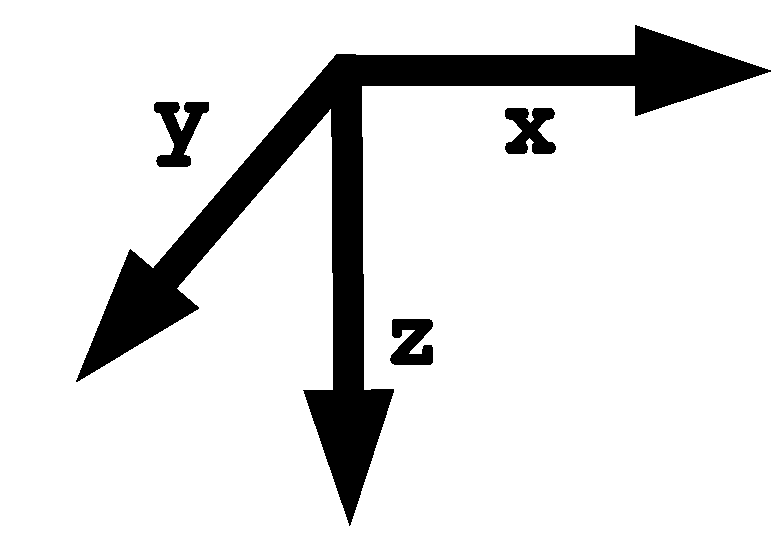
\includegraphics[height=0.2\linewidth]{rightHandedCoord.ps}
  \caption{\emph{SW4} uses a right handed coordinate system with the z-axis pointing
  downwards.}
  \label{fig:coordsys}
\end{centering}
\end{figure}
\emph{SW4} employs MKS (meters-kilograms-seconds) units. All distances (e.g.,~grid dimensions,
spacing, and displacements) are in meters (m), time is in seconds (s), seismic P- and S-wave
velocities are in meters per second (m/s), densities are in kilogram per cubic meter (kg/m$^3$),
forces are in Newton (N), and seismic moment (torque) is in Newton-meters (Nm). All angles
(e.g. latitude, longitude, azimuth, strike, dip and rake) are in degrees. 
%The quality factors $Q_P$ and $Q_S$ are dimensionless.

In \emph{SW4} the computational domain is rectangular in the horizontal plane,
\[
0\leq x\leq x_{max},\quad 0\leq y\leq y_{max}.
\]
The topography surface
\[
z=\tau(x,y),
\]
defines the shape of the top surface in the vertical direction. \emph{SW4} can also be run without
topography. In that case, $\tau(x,y)=0$. The computational domain is given by
\begin{equation}\label{eq:domain}
0\leq x\leq x_{max},\quad 0\leq y\leq y_{max},\quad \tau(x,y) \leq z \leq z_{max}.
\end{equation}
The grid command in the input file specifies the extent of the computational domain and the grid
size $h$. When mesh refinement is enabled, this is the grid size in the coarsest grid. The most
obvious way of specifying the grid is by providing the number of grid points in each direction as
well as the grid size,
%
\begin{verbatim}
	grid nx=301 ny=201 nz=101 h=500.0 
\end{verbatim}
%
This line gives a grid with grid size 500 meters, which extends 150 km in $x$, 100 km in $y$ and 50 km in the
$z$-direction. Alternatively, the grid can be specified by giving the spatial range in each of the three
dimensions and explicitly specifying the grid spacing. For example,
%
\begin{verbatim}
	grid x=30e3 y=20e3 z=10e3 h=500.0 
\end{verbatim}
%
results in a grid which spans 30,000 meters in $x$, 20,000 meters in $y$, and 10,000
meters in the $z$-direction.  The grid spacing is 500 meters, which is used to compute the
number of grid points in each direction: nx=61, ny=41, and nz=21, for a total of
52,521 grid points. Note that the number of grid points in the different directions will be
rounded to the nearest integer value according to the pseudo C-code
\begin{equation}\label{eq:nx-calculation}
nx = \mbox{(int)} (1.5 + x/h).
\end{equation}
The extent in the $x$-direction is thereafter adjusted to
\begin{equation}\label{eq:x-calculation}
x=(nx-1) h.
\end{equation}
A corresponding procedure is performed in the other coordinate directions.

The third option is to give the spatial range in each of the three dimensions and specify the number
of grid points in a particular direction:
%
\begin{verbatim}
	grid x=30000 y=20000 z=10000 nx=100
\end{verbatim}
%
In this case, the grid spacing is computed as 
\[
h = x/(nx-1)= 303.03.
\]
Note that no rounding needs to take place in this case, since $h$ is a floating point number. Given this
value of $h$, ny and nz are computed using formulas corresponding to
(\ref{eq:nx-calculation}) giving ny=34 and nz=67, for a total of 227,800 grid points. Again,
the extents in the $y$ and $z$-directions are adjusted corresponding to (\ref{eq:x-calculation}). The syntax
for the grid command is given in Section~\ref{keyword:grid}.

The simulation always starts at $t=0$ and runs until $t=T$, where $T$ is the user specified end
time.  The {\tt time} command specifies the end time. For example,
\begin{verbatim}
time t=1.6
\end{verbatim}
sets $T=1.6$ seconds. Alternatively, the simulation time interval can be specified as 
a number of time steps, as in the example
\begin{verbatim}
time steps=1200
\end{verbatim}
Here the number of time steps is set to 1200. The end time will in this case be $T=1200\Delta t$, where the
time step $\Delta t$ depends on the input material. $\Delta t$ is determined automatically by \emph{SW4}.
The simulation start time can be related to a UTC time. The option {\tt utcstart} sets the UTC time that
corresponds to the simulation time $t=0$, for example,
\begin{verbatim}
time t=1.6 utcstart=01/31/2012:17:34:12.233
\end{verbatim}
The format of the UTC time is ``month/day/year:hour:minute:second.millisecond''. When the UTC time
is set, it is saved in the header of all output receiver data files. Note that the UTC start time
is essential for correctly aligning observed data when solving the inverse problem with \emph{SW4opt}.

\section{Geographical coordinates and projections}
\index{geographical coordinates}
\begin{figure}
\begin{centering}
  \includegraphics[width=0.6\linewidth]{LatLonAz.ps}
%  \includegraphics{LatLonAz.ps}
  \caption{Geographical coordinates in \emph{SW4}.}
  \label{fig:geocoord}
\end{centering}
\end{figure}
\emph{SW4} supports geographical coordinates as an alternative way of specifying spatial locations,
see Figure~\ref{fig:geocoord}. The geographic location of the origin of the Cartesian coordinte
system (lat$_0$, lon$_0$) is specified in the grid command, and if no location is given it defaults
to lat$_0$ = 37 degrees (North), lon$_0$ = -118 degrees (West), with a 135 degree azimuthal angle
between North and the $x$-axis. The vertical coordinate is zero ($z=0$) at mean sea level. 

\subsection{Spheroidal mapping}
By default, the latitude (lat) and longitude (lon) are calculated using a spheroidal mapping,
\begin{alignat}{2}
\mbox{lat} &= \mbox{lat$_0$} + \frac{x\cos(\alpha) - y\sin(\alpha)}{M},\quad \alpha =
\mbox{az}\frac{\pi}{180}, \label{eq:lat}\\
\mbox{lon} &= \mbox{lon$_0$} + \frac{x\sin(\alpha ) + y\cos(\alpha)}{M\cos(\phi \pi/180)}.\label{eq:lon}
\end{alignat}
In this formula, lat, lon, az, lat$_0$, and lon$_0$ are all in degrees, and $M = 111,319.5$
meters\footnote{Note that $M/60 = 1,855.325$ meters corresponds to one minute of arc of
  longitude along the Equator on the WGS84 ellipsoid. This distance is also known as a geographical
  mile and is approximately equal to a Nautical mile (1,852 meters).}.  You can change the location
and orientation of the grid by specifying the latitude and longitude of the grid origin, as well as
the azimuthal angle between North and the $x$-axis. For example:
\begin{verbatim}
grid h=500 x=30000 y=20000 z=10000 lat=39 lon=-117 az=150
\end{verbatim}
sets the origin of the grid to latitude 39 degrees (North), longitude -117 degrees
(West), and azimuthal angle 150 degrees.

The default projection is spheriodal as described by equations \eqref{eq:lat}-\eqref{eq:lon}. You
can change the parameter $M$ with the {\bf mlat} keyword in the {\bf grid} command. By using the
{\bf mlon} keyword, you can also modify the projection by replacing $M\cos(\phi\pi/180)$ in
\eqref{eq:lon} by the constant value $M_{lon}$. Using the {\bf mlon} keyword is only recommended if
the computational domain is small and accurate values of both {\bf mlon} and {\bf mlat} are
available.

\subsection{The Proj.4 library}
More accurate projections are available through the Proj4 library (if
\emph{SW4} was built with Proj4 support). These projections are enabled by using the {\bf proj}
and/or {\bf ellps} keywords in the {\bf grid} command. For example,
\begin{verbatim}
grid h=300 x=40e3 y=43e3 z=40e3 lat=45.01 lon=5.52 az=0 proj=utm ellps=WGS84
\end{verbatim}
sets the origin of the grid to latitude 45.01 degrees (North), longitude 5.52 degrees (East), and
azimuthal angle 0. Here we use the UTM projection based on the WGS84 ellipse. Note that the strings
``proj=utm'' and ``ellps=WGS84'' are passed directly to the Proj4 library to initialize the
projection. Many other options are available. See the Proj4 documentation~\cite{Proj4} for further
details.

\section{Super-grid damping layers}

\emph{SW4} implements a super-grid modeling technique to reduce artificial reflections from the
far-field boundaries~\cite{AppCol-09, PetSjo-13}. In this method, a coordinate mapping (stretching
function) is used to map the computational domain to a much larger physical domain. A high order
artificial dissipation operator is added in the super-grid layers. The ideas behind the super-grid
technique are to slow down the waves as they propagate through the layer, and to damp them out
before they arrive at the outer boundary of the computational domain. Note that the dissipative term
is only added in the layers, and should not affect the accuracy in the interior of the domain.

The coordinate stretching compresses the solution inside the layers. This corresponds to a slowing
down of all traveling waves in the direction normal to each far-field boundary. As a result, the
isotropic elastic wave equation becomes anisotropic in the super-grid layers. It is possible to
prove by energy estimates that the super-grid modeling leads to a stable numerical method with
decreasing energy. This estimate is valid for heterogeneous material properties and free surface
boundary conditions on one or more sides of the domain. See the paper by Petersson and
Sjogreen~\cite{PetSjo-13} for more details.

Super-grid layers are included on all sides of the computational domain, except along the
free surface, see Figure~\ref{fig:layout}.
\begin{figure}[th]
\begin{center}
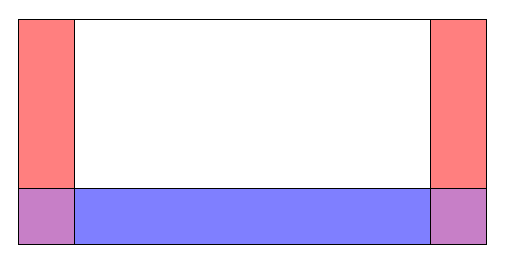
\includegraphics[width=0.65\linewidth]{layout.eps}
%\includegraphics[width=0.65\linewidth]{layout.png}
\caption{\em A vertical cross-section through the computational domain with a free surface boundary
  along the top edge. The original seismic wave equation is solved the white region. The wave speed
  is reduced in the normal direction of the surrounding super-grid layers, where also a high order
  damping term is added.}\label{fig:layout}
\end{center}
\end{figure}
The default thickness of the layers (currently) equals 30 grid sizes. The thickness of the
super-grid layers can be changed with the {\tt supergrid} command, see Section~\ref{sec:supergrid}.

For practical reasons, the super-grid layers are part of the computational domain as specified by
the grid command. If, for example, each super-grid layer is 30 grid points wide, the solution
should be considered artificial in the first and last 30 points in each horizontal direction, and
the bottom 30 points in the vertical direction. Note that the numerical solution within the layers
do {\em not} approximate the solution of the seismic wave equation. For this reason, it is important
to make the computational domain sufficiently large. If the super grid layers are 30 grid points
wide, the computational grid must be at least 60 grid points wide in the $x$ and $y$-directions, and
30 points wide in the Cartesian part of the $z$-direction. Additional grid points must be added in
the interior of the computational domain for the actual seismic modeling. Note that sources and
receivers should only be placed in the interior of the computational domain, i.e., away from the
super-grid layers.

%%%%%%%%%%%%%%%%%%%%%%%%%%%%%%%%%%%%%%%%%%%%%%%%
\chapter{Sources, time-functions and grid sizes}
%%%%%%%%%%%%%%%%%%%%%%%%%%%%%%%%%%%%%%%%%%%%%%%%

The source time function can be selected from a set of predefined functions, or by spline
interpolation of a user defined discrete time-series. Each point force or point moment tensor source
can have a different time function. 

\section{Predefined time functions}\label{sec:predefined}

All pre-defined source time functions start from zero ($\lim_{t\to -\infty} g(t,t_0,\omega) = 0$) and tend to a constant terminal
value, $\lim_{t\to \infty} g(t,t_0,\omega) = g_\infty$. In seismic applications, $g_\infty\ne 0$
usually corresponds to solving for the displacements of the motion, because the solution will tend to
a non-zero steady state solution for large times. This solution corresponds to the final
displacements due to a seismic event. When $g_\infty = 0$, the solution will always tend to zero for
large times, as is expected from the velocities or accelerations of the motion due to a seismic event.

The Gaussian, Dirac, and Triangle functions integrate to one ($\int_{-\infty}^{\infty}
g(t,t_0,\omega) \, dt = 1$), while the Sawtooth, Smoothwave, and Ricker functions integrate to zero
and have maximum amplitude one. The RickerInt function is the time-integral of the Ricker function
and integrates to zero. The GaussianInt, Brune, BruneSmoothed, and Liu functions tend to one
($\lim_{t\to\infty} g(t,t_0,\omega) = 1$).

The Triangle, Sawtooth, Ramp, Smoothwave, Brune, BruneSmoothed, Liu and VerySmoothBump functions are
identically zero for $t<t_0$, so they will give reasonable simulation results if $t_0\geq
0$. However, the Gaussian, GaussianInt, Ricker, and RickerInt functions are centered around $t=t_0$
with exponentially decaying tails for $t<t_0$. Hence $t_0$ must be positive and of the order ${\cal
  O}(1/\omega)$ to avoid incompatibilty problems with the initial conditions. We recommend choosing
$t_0$ such that $g(0,t_0,\omega) \leq 10^{-8}$ for these functions.

\subsection{Gaussian}\label{gaussian}
  \[
  g(t,t_0,\omega) = \dfrac{\omega}{\sqrt{2 \pi}} e^{-\omega^2 (t - t_0)^2 /2}.
  \] 
Note that the spread of the Gaussian function (often denoted $\sigma$) is related to $\omega$ by
$\sigma = 1 / \omega$. A plot of the Gaussian time-function is shown in Figure~\ref{fig:gaussians}.

\subsection{GaussianInt (or Erf)}\label{gaussianint}
\[
g(t,t_0,\omega) = \dfrac{\omega}{\sqrt{2 \pi}} \int_{-\infty}^t e^{-\omega^2 (\tau - t_0)^2/2}\,d\tau.
\] 
GaussianInt is the time-integral of the Gaussian. A plot of the
GaussianInt time-function is shown in Figure~\ref{fig:gaussians}.
\begin{figure}
\begin{centering}
  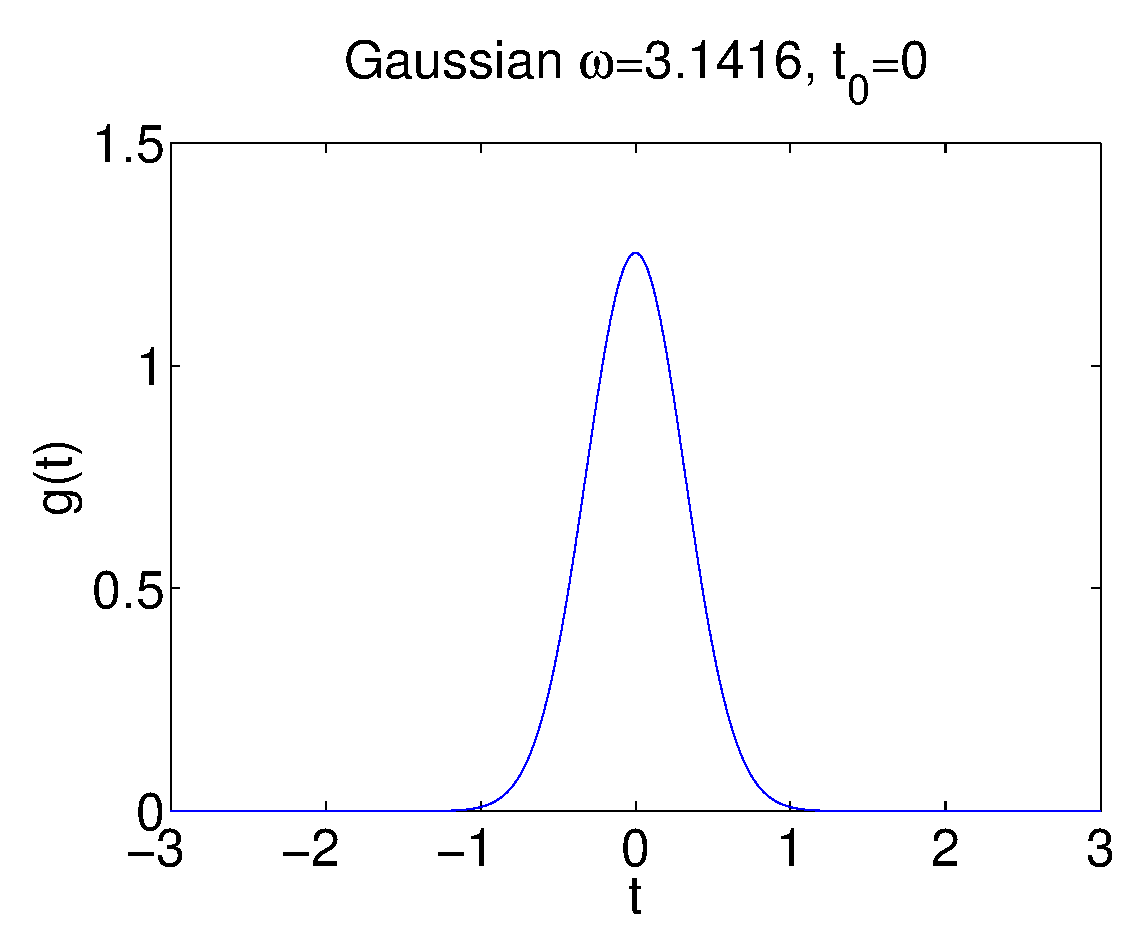
\includegraphics[width=0.4\linewidth]{f1-gaussian.ps}
  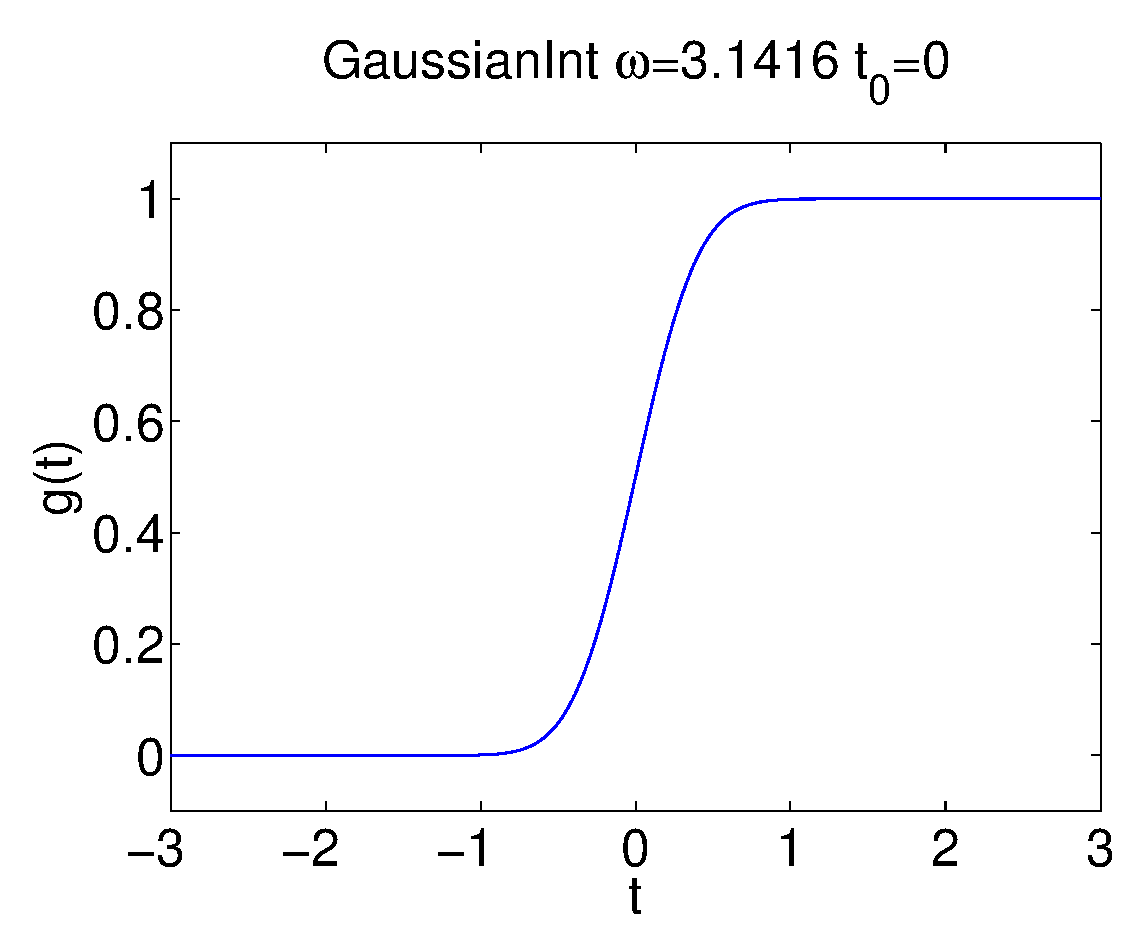
\includegraphics[width=0.4\linewidth]{f2-gaussianint.ps}
  \caption{Gaussian (left) and GaussianInt (right) with $\omega=\pi$ and $t_0=0$.}
  \label{fig:gaussians}
\end{centering}
\end{figure}  
%
\subsection{Ricker} \label{ricker}
  \[
  g(t,t_0,\omega) = \left(2 \pi^2 \omega^2 (t - t_0)^2 - 1\right) e^{- \pi^2 \omega^2 (t - t_0)^2}.
  \]
A plot of the Ricker time-function is shown in Figure~\ref{fig:rickers}.
\subsection{RickerInt}\label{rickerint}
  \[
  g(t,t_0,\omega) = (t - t_0) e^{- \pi^2 \omega^2 (t - t_0)^2}.
  \]
RickerInt is the time integral of the Ricker function, and is proportional to the time-derivative of
the Gaussian function. Since the RickerInt function tends to zero for large times, it does not lead
to any permanent displacements. A plot of the RickerInt time-function is shown in
Figure~\ref{fig:rickers}.
\begin{figure}
\begin{centering}
  \includegraphics[width=0.4\linewidth]{f3-ricker.ps}
  \includegraphics[width=0.4\linewidth]{f4-rickerint.ps}
  \caption{Ricker (left) and RickerInt (right) with $\omega=1$ and $t_0=0$.}
  \label{fig:rickers}
\end{centering}
\end{figure}  
%
\subsection{Brune} 
 \label{brune}
\[
 g(t,t_0,\omega) = \left\{
\begin{array}{ll} 
0, & t < t_0, \\ 
1 - e^{-\omega(t-t_0)}( 1+\omega(t-t_0) ), & t \geq t_0.
\end{array}
\right.
\]
Note that the Brune function only has one continuous derivative. Because its second derivative is discontinuous at
$t=t_0$, this function can generate noisy numerical solutions. We recommend filtering all computed time
series, or using the {\bf prefilter} command to remove any unresolved motions.

\subsection{BruneSmoothed}
The BruneSmoothed function has three continuous derivatives at $t=t_0$, but is otherwise similar to
the Brune function,
\[
 g(t,t_0,\omega) = \left\{
\begin{array}{ll} 
0, & t < t_0, \\ 
1 - e^{-\omega(t-t_0)}\left[ 1+\omega(t-t_0) + \dfrac{1}{2}(\omega(t-t_0))^2\right. & \\
\quad \left.-\,\dfrac{3}{2\tau_0}( \omega(t-t_0))^3  + \dfrac{3}{2\tau_0^2}( \omega(t-t_0))^4 -
 \dfrac{1}{2\tau_0^3}( \omega(t-t_0))^5 \right], & 0< \omega (t-t_0) < \tau_0,\\
1 - e^{-\omega(t-t_0)}( 1+\omega(t-t_0) ), & \omega (t-t_0) > \tau_0.
\end{array}
\right.
\]
The parameter $\tau_0$ in the above formula is fixed to the value $2.31$. Plots of the Brune and
BruneSmoothed time-functions are shown in Figure~\ref{fig:brunes}. Since the BruneSmoothed function
has three continuous derivatives, it generates less high frequency noise than the Brune function and
gives better accuracy for a given grid resolution.
\begin{figure}
\begin{centering}
  \includegraphics[width=0.4\linewidth]{f9-brune.ps}
  \includegraphics[width=0.4\linewidth]{f10-brunesmoothed.ps}
  \caption{Brune (left) and BruneSmoothed (right) with $\omega=2$ and $t_0=-1$.}
  \label{fig:brunes}
\end{centering}
\end{figure}  

\subsection{Liu}
\renewcommand{\arraystretch}{1.5}
This function was given in the paper by Liu et al., \cite{liuetal_2006}. 
It is defined by 
\[
g(t,t_0,\omega) = \left\{ 
\begin{array}{ll}
  0, & t \leq t_0, \\
  C\left[0.7(t-t_0) + \dfrac{1.2}{\pi}\tau_1 - \dfrac{1.2}{\pi}\tau_1
  \cos\left(\dfrac{\pi (t-t_0)}{2\tau_1}\right) \right. & \\
     \hfill \left. -\,\dfrac{0.7}{\pi}\tau_1\sin\left(\dfrac{\pi (t-t_0)}{\tau_1}\right)\right],  & 
     t_0 < t \leq \tau_1+t_0, \\
%
  C\left[t-t_0-0.3\tau_1+\dfrac{1.2}{\pi}\tau_1-\dfrac{0.7}{\pi}\tau_1\sin\left(\dfrac{\pi
    (t-t_0)}{\tau_1}\right)\right. & \\ 
    \hfill
    \left. +\,\dfrac{0.3}{\pi}\tau_2\sin\left(\dfrac{\pi(t-t_0-\tau_1)}{\tau_2}\right)\right], &  
    \tau_1+t_0 < t \leq 2\tau_1+t_0, \\
%
  C\left[0.3(t-t_0)+1.1\tau_1+\dfrac{1.2}{\pi}\tau_1\right. & \\
    \hfill
    \left. +\,\dfrac{0.3}{\pi}\tau_2\sin\left(\dfrac{\pi(t-t_0-\tau_1)}{\tau_2}\right)\right], & 
    2\tau_1+t_0 < t \leq \tau+t_0, \\
  1,  &  t > \tau +t_0.
\end{array} \right.
\]
\noindent The parameters are given by $\tau=2\pi/\omega$, $\tau_1=0.13\tau$, $\tau_2 = \tau-\tau_1$,
and $C=\pi/(1.4\tau_1\pi+1.2\tau_1+0.3\tau_2\pi)$.  The Liu function resembles the Brune function,
but the rise is somewhat steeper for small $t-t_0$, see Figure~\ref{fig:liu}.
\begin{figure}
\begin{centering}
  \includegraphics[width=0.4\linewidth]{f12-liu.ps}
  \caption{Liu time function with $\omega=2$ and $t_0=0$.}
  \label{fig:liu}
\end{centering}
\end{figure}  

\subsection{Triangle}
\renewcommand{\arraystretch}{1.3}
For $ t_0 < t < t_0 + 1/\omega$,
\[
  g(t,t_0,\omega) = \dfrac{16 \omega}{\pi^2} \left[ \sin(\pi\omega(t - t_0)) - \dfrac{\sin(3 \pi
      \omega(t - t_0))}{9} + \dfrac{\sin(5 \pi \omega(t - t_0)}{25} - \dfrac{\sin(7 \pi \omega(t -
      t_0))}{49}\right],
\] 
with $g(t,t_0,\omega) = 0$ elsewhere. A plot of the Triangle time-function is shown in
Figure~\ref{fig:triandsaw}.
%
\subsection{Sawtooth}
For $ t_0 < t < t_0 + 1/\omega$,
\[
  g(t,t_0,\omega) = \dfrac{8}{\pi^2} \left[\sin(2 \pi \omega (t - t_0) ) - \dfrac{\sin(6 \pi
      \omega(t - t_0))}{9} + \dfrac{\sin(10 \pi \omega (t - t_0) )}{25} - \dfrac{\sin(14 \pi
      \omega(t - t_0 ))}{49}\right],
\]
with $g(t,t_0,\omega) = 0$ elsewhere.  A plot of the Sawtooth time-function is shown in
Figure~\ref{fig:triandsaw}.
\begin{figure}
\begin{centering}
  \includegraphics[width=0.4\linewidth]{f5-triangle.ps}
  \includegraphics[width=0.4\linewidth]{f6-sawtooth.ps}
  \caption{Triangle (left) and Sawtooth (right) with $\omega=1$ and $t_0=0$.}
  \label{fig:triandsaw}
\end{centering}
\end{figure}  
%
\subsection{Ramp}
\[ 
g(t,t_0,\omega) = \left\{ 
\begin{array}{ll} 
0, & t < t_0,\\
0.5 (1 - \cos(\pi (t - t_0) \omega)),& t_0 \leq t \leq t_0 + 1/\omega,\\
1, & t > t_0 + 1/\omega.
\end{array}
\right.
\]
A plot of the Ramp time-function is shown in Figure~\ref{fig:rampandsmoothwave}.
%
\subsection{Smoothwave}
For $ t_0 < t < t_0 + 1/\omega$,
\begin{multline*}
 g(t,t_0,\omega) = \dfrac{2187}{8} (\omega(t-t_0))^3 - \dfrac{10935}{8} (\omega(t - t_0))^4  +
  \dfrac{19683}{8} (\omega(t - t_0))^5\\ - \dfrac{15309}{8} (\omega(t - t_0))^6 +
  \dfrac{2187}{4}(\omega(t - t_0))^7,
\end{multline*}
with $g(t,t_0,\omega) = 0$ elsewhere. A plot of the Smoothwave time-function is shown in
Figure~\ref{fig:rampandsmoothwave}.
\begin{figure}
\begin{centering}
  \includegraphics[width=0.4\linewidth]{f7-ramp.ps}
  \includegraphics[width=0.4\linewidth]{f8-smoothwave.ps}
  \caption{Ramp (left) and Smoothwave (right) with $\omega=1$ and $t_0=0$.}
  \label{fig:rampandsmoothwave}
\end{centering}
\end{figure}  
%
\subsection{VerySmoothBump} 
\[
g(t,t_0,\omega) = \left\{ 
\begin{array}{ll} 
0, & t < t_0,\\ 
1024\,\omega^5(t-t_0)^5 (1 - \omega(t-t_0))^5,& t_0 \leq t \leq t_0+1/\omega,\\ 
0, & t > t_0 + 1/\omega.
\end{array}
\right.
\]
The VerySmoothBump function satisfies $0\leq g\leq 1$. It has four continuous derivatives.
A plot of the VerySmoothBump time-function is shown in Figure~\ref{fig:verysmoothbump}.
\begin{figure}
\begin{centering}
  \includegraphics[width=0.4\linewidth]{f11-verysmoothbump.ps}
  \caption{VerySmoothBump with $\omega=0.5$ and $t_0=0$.}
  \label{fig:verysmoothbump}
\end{centering}
\end{figure}  
%
\subsection{C6SmoothBump} 
\[
g(t,t_0,\omega) = \left\{ 
\begin{array}{ll} 
0, & t < t_0,\\ 
51480\, \omega^7 (t-t_0)^7 (1- \omega(t-t_0))^7, & t_0 \leq t \leq t_0 + 1/\omega,\\ 
0, & t > t_0 + 1/\omega.
\end{array}
\right.
\]
The C6SmoothBump function has six continuous derivatives and integrates to one.
A plot of the C6SmoothBump time-function is shown in Figure~\ref{fig:c6smoothbump}.
\begin{figure}
\begin{centering}
  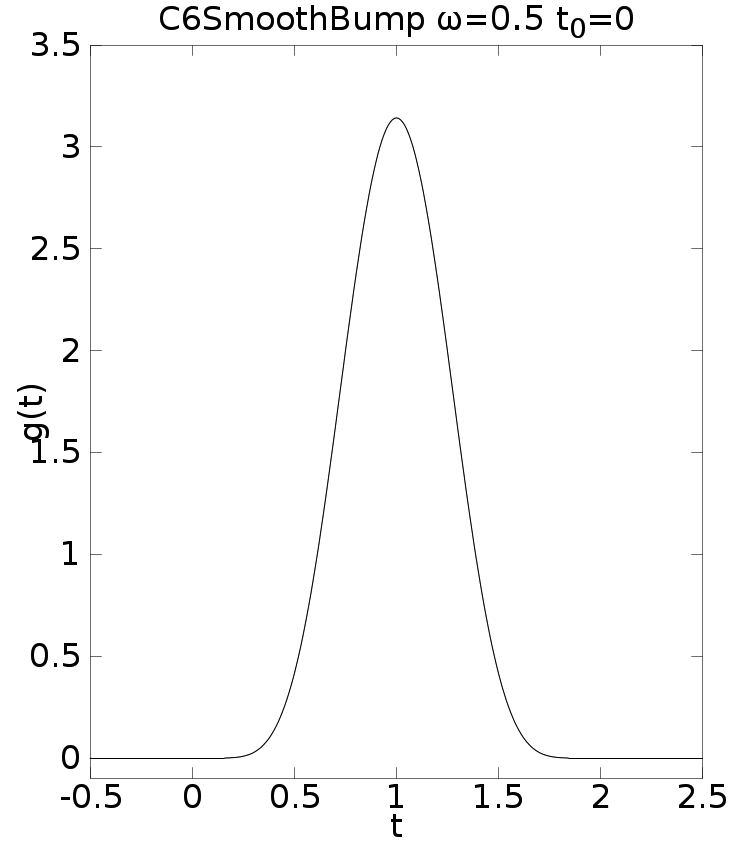
\includegraphics[width=0.9\linewidth]{f12-c6smoothbump.eps}
  \caption{C6SmoothBump with $\omega=2$ and $t_0=0$.}
  \label{fig:c6smoothbump}
\end{centering}
\end{figure}  
%
\subsection{GuassianWindow}
\[
g(t,t_0,\omega) = \sin(\omega t) e^{-(\omega(t-t_0)/N_c)^2/2}
\]
A plot of the GaussianWindow time-function with $N_c=5$ is shown in
Figure~\ref{fig:gaussianwindow}. Note that $N_c$ is specified with the \verb+ncyc+ keyword, which
must be given when this time function is used in the \verb+source+ command.
\begin{figure}
\begin{centering}
  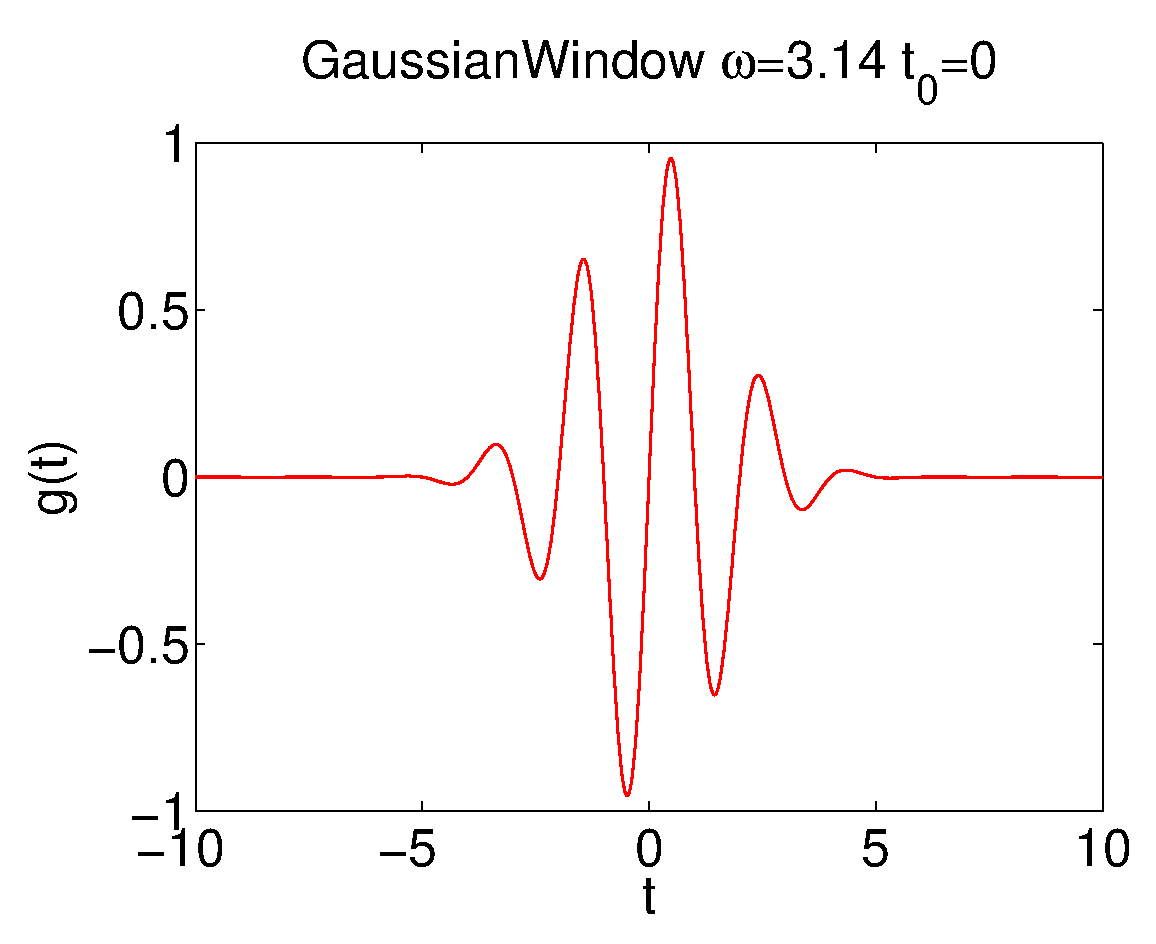
\includegraphics[width=0.6\linewidth]{GW.eps}
  \caption{GaussianWindow with $\omega=3.14$, $t_0=0$, and $N_c=5$.}
  \label{fig:gaussianwindow}
\end{centering}
\end{figure}  

\subsection{Dirac}
The Dirac distribution $\delta(t-t_0)$ is not a regular function because it is zero everywhere,
except at $t=t_0$ where it is undefined. The integral of $\delta(t)$ is one. If $f(t)$ is a smooth
function, then
\begin{equation}\label{eq:dirac}
\int f(t)\delta(t-\tau)\, dt = f(\tau).
\end{equation}
We discretize the Dirac distribution on a grid $t_n = n\Delta_t$, where $\Delta_t>0$ is the constant
time step used by the solver of the elastic wave equation. We obtain the discrete time series $d_n$,
$n=0,1,2,\ldots$ by imposing moment conditions such that \eqref{eq:dirac} is satisfied for all
polynomial functions $f(t)=t^q$, $q=0,1,\ldots,Q$, in the sense
\[
\Delta_t \sum_{n=0}^\infty d_n t_n^q = \tau^q,\quad q=0,1,\ldots,Q. 
\]
This leads to $Q+1$ conditions for the coefficients $d_n$. The specification of $d_n$ is made unique
by enforcing $d_n=0$ except at $Q+1$ consecutive grid points surrounding $t=\tau$. This procedure is
similar to our spatial discretization of point force and moment tensor sources, see~\cite{PetSjo-10}
for details.

The discretized Dirac distribution triggers all frequencies on the mesh, including completely
unresolved and unphysical motions. The numerical solution is therefore meaningless unless it is
filtered to remove the unresolved motions. The filtering can either be done after the simulation is
completed, or by using the {\bf prefilter} command.

\section{Discrete time function}

The discrete time function constructs a quintic (5th order) spline function that interpolates the
given function values $g_j = g(\tau_j)$, for $j=1,2,\ldots, N_s$, where $N_s\geq 7$. The function
values are specified on an equidistant grid, $\tau_j = t_0 + (j-1) \delta_t$, where
$\delta_t>0$. Note that the time step can be chosen independently of the time step in the solver of
the elastic wave equation. The start time, $t_0$, can also have an arbitrary value. The
interpolation procedure results in six polynomial coefficients for each interval $\tau_j\leq t
<\tau_{j+1}$. The coefficients are chosen such that g(t) becomes four times continuously
differentiable.

Because the elastic wave equation is solved for $0\leq t\leq T$, it is necessary to evaluate the
discrete time function in this interval. If $t_0>0$, the discrete time function uses the polynomial
coefficients corresponding to the first interval $[\tau_1,\tau_2]$ for all $t<t_0$. Similarily,
if $\tau_{N_s}<T$, the coefficients for the last interval are used for $t>\tau_{N_s}$. To avoid
unexpected results due to extrapolation, we recommend specifying the discrete time function for all
$t\in[0,T]$. To also avoid incompatibilities between the forcing and the homogeneous initial conditions,
we recommend setting $g_j=0$ for all $\tau_j\leq 0$.

The file format for discrete time functions is decribed in~\ref{sec:discrete-time-function-format}.

\section{How fine does the grid need to be?}\label{sec:grid-size}
\index{grid size}

When preparing the input file, the most difficult parameter to choose is probably the grid size
$h$. It is extremely important to use a grid size which is sufficiently small, because you must resolve
the waves that are generated by the source. On the other hand you don't want to use an
unnecessarily small grid size, because both the execution time and the memory requirements
increase with decreasing grid size, see Section~\ref{sec:performance}.

WHERE TO PUT THIS?  We have compared \emph{SW4} and \emph{WPP} on problems where the exact solution
is known. Compared to \emph{WPP}, \emph{SW4} gives similar accuarcy with significantly fewer grid
points per wave length. This means that waves with the same frequency can be resolved on a grid that
is coarser both in space and time. For materials with $C_p/C_s\approx 2$ and an accuracy of about 10
percent, the \emph{SW4} code calculates the solution about eight times faster than \emph{WPP}, using
about one eighth of the memory. When both codes use the same grid size, \emph{SW4} can capture waves
with approximately twice as high frequency.

The number of grid points per shortest wavelength, $P$, is a normalized measure of how well a
solution is resolved on the computational grid. Since the shear waves have the lowest velocities and
a shorter wave length than the compressional waves, the shortest wave length $L_{min}$ can be
estimated by
\[
 L_{min} = \dfrac{\min V_s}{f_{max}},
\]
where $V_s$ is the shear velocity of the material and $f_{max}$ is the largest significant frequency
in the time function $g(t)$. Hence the number of grid points per wave length equals $L_{min}/h$,
which is given by
%
\begin{equation}\label{eq:resolutionformula}
  P = \dfrac{\min V_s}{h\,f_{max}}. 
\end{equation}
Note that $h$ needs to be made smaller to maintain the same value of $P$ if either $V_s$ is
decreased or if the frequency is increased. In formula (\ref{eq:resolutionformula}), $\min V_s$ is
found from the material properties and $h$ is determined by the input grid specification.  The
frequency spectrum of the solution is determined by the frequency spectrum of the time
function(s) in the source term(s).

Figure~\ref{fig:fouriers} displays the absolute values of the Fourier transforms of the
functions Gaussian, RickerInt, Ricker, and the time derivative of the Brune
function. Inspection of the mathematical definitions of the Gaussian and Brune functions
shows that the {\tt freq} parameter specifies the angular frequency for these
functions. The relation between the fundamental frequency $f_0$ and the {\tt freq} parameter is
given by
\begin{equation}\label{eq:angular-scaling}
f_0 = \left\{ \begin{array}{ll}
 {\tt freq},& \mbox{for Ricker, RickerInt, and VerySmoothBump},\\
 \dfrac{\tt freq}{2\pi},& \mbox{for Liu, Brune, BruneSmoothed, Gaussian, GaussianInt, and GaussianWindow}.
\end{array}\right.
\end{equation}
The plots in Figure~\ref{fig:fouriers} were made with frequency parameter {\tt freq}=0.25 for the
Ricker and RickerInt functions and frequency parameter {\tt freq}=1.5 for the Gaussian and
$d/dt$(Brune) functions. Hence, $f_0\approx 0.25$ for all functions in
Figure~\ref{fig:fouriers}. Note that the Fourier
transform of the Brune function decays much slower than the other functions for high
frequencies. This is due to its lack of smoothness at $t=t_0$.
\begin{figure}
\begin{center}
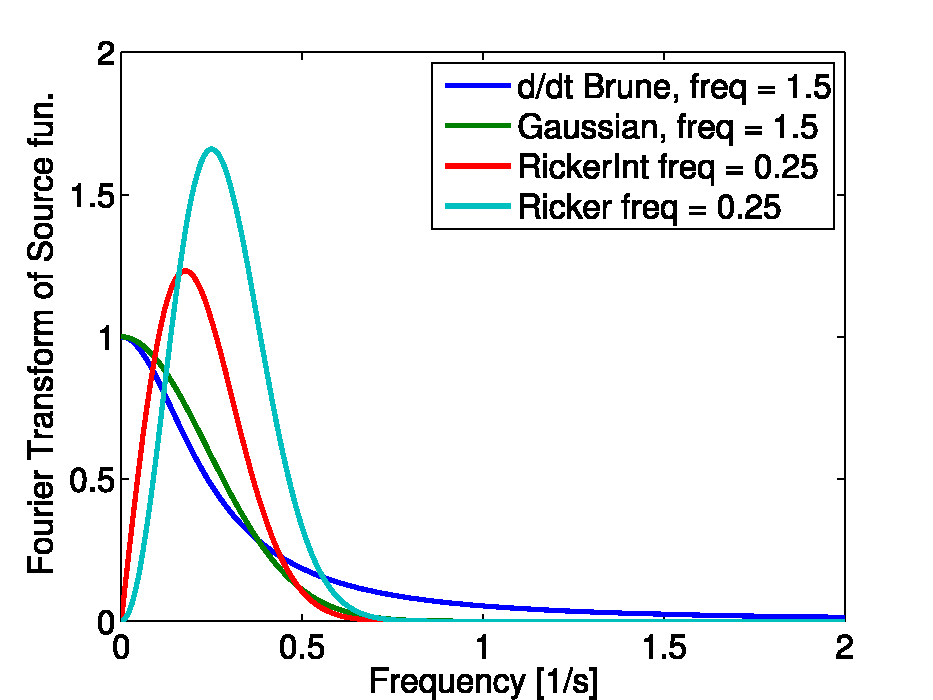
\includegraphics[width=0.6\textwidth]{figfouriers.ps}
\caption{ Magnitude of the Fourier transform of the derivative of the Brune (dark
  blue), the Gaussian (green), the RickerInt (red), and the Ricker (light blue)
  time-functions. Here {\tt freq}=1.5 for the Gaussian and the derivative of the Brune
  function, and {\tt freq}=0.25 for Ricker and RickerInt.}
\label{fig:fouriers}
\end{center}
\end{figure}

It is the upper power (highest significant) frequency in the time function that shall be used in
(\ref{eq:resolutionformula}) to estimate the number of grid points per wave length. For practical
purposes $f_{max}$ can be defined as the frequency where the amplitude of the Fourier
transform falls below 5 \% of its max value. We have
\begin{equation}\label{eq:upper-power-freq}
f_{max} \approx \begin{cases}2.5 f_0,&\mbox{Ricker, RickerInt, Gaussian time functions},\\
  4 f_0,&\quad\mbox{Brune time function}.
\end{cases}
\end{equation}
In other words, simulations using the Brune function are harder to resolve on the grid and need much
more grid points to give reliable results.

Our experience is that \emph{SW4} gives accurate results for 
\[
P \geq ??,
\]
but the exact number depends on the distance between the source and the reciever. Note that the
relation between the fundamental frequency $f_0$ and the upper power frequency $f_{max}$ in
(\ref{eq:upper-power-freq}) is very important. For other time functions, $f_{max}$ can be estimated
using the matlab/octave scripts fcnplot and ftfcnplot in the {\tt tools} directory. A lower number
for $P$ can be used in some practical situations. The best way of checking the accuracy in
a numerical solution is to repeat the calculation on a finer mesh, even though this approach
can become computationally expensive. 

We finally remark that the ratio between the compressional and shear velocity, $V_P/V_S$, can have a
significant influence on the accuracy of surface waves, see the paper by Kreiss and
Petersson~\cite{KrePet-12} for details.


%%%%%%%%%%%%%%%%%%%%%%%%%%%%%%%%%%%%%%%%%%%%%%%%
\chapter{The material model (not documented)} \label{sec:material}

%%%%%%%%%%%%%%%%%%%%%%%%%%%%%%%%%%%%%%%%%%%%%%%%
\chapter{Topography (not documented)} \label{sec:topography}
%%%%%%%%%%%%%%%%%%%%%%%%%%%%%%%%%%%%%%%%%%%%%%%%

%%%%%%%%%%%%%%%%%%%%%%%%%%%%%%%%%%%%%%%%%%%%%%%%
%\chapter{Mesh refinement} \label{sec:mesh-ref}
%%%%%%%%%%%%%%%%%%%%%%%%%%%%%%%%%%%%%%%%%%%%%%%%

%%%%%%%%%%%%%%%%%%%%%%%%%%%%%%%%%%%%%%%%%%%%%%%%
%\chapter{Attenuation}\label{sec:attenuation}
%%%%%%%%%%%%%%%%%%%%%%%%%%%%%%%%%%%%%%%%%%%%%%%%

%%%%%%%%%%%%%%%%%%%%%%%%%%%%%%%%%%%%%%%%%%%%%%%%
\chapter{Output options (not documented)}
%%%%%%%%%%%%%%%%%%%%%%%%%%%%%%%%%%%%%%%%%%%%%%%%

%%%%%%%%%%%%%%%%%%%%%%%%%%%%%%%%%%%%%%%%%%%%%%%%
\chapter{Examples (not documented)} \label{sec:examples}
%%%%%%%%%%%%%%%%%%%%%%%%%%%%%%%%%%%%%%%%%%%%%%%%

%%%%%%%%%%%%%%%%%%%%%%%%%%%%%%%%%%%%%%%%%%%%%%%%
\chapter{Keywords in the input file (in progress)}\label{chap:keywords}
%%%%%%%%%%%%%%%%%%%%%%%%%%%%%%%%%%%%%%%%%%%%%%%%
The syntax of the input file is
\begin{verbatim}
command1 parameter1=value1 parameter2=value2 ... parameterN=valueN
# comments are disregarded
command2 parameter1=value1 parameter2=value2 ... parameterN=valueN
...
\end{verbatim}
Each command starts at the beginning of the line and ends at the end of the same line. Blank and
comment lines are disregarded. A comment is a line starting with a \# character. The order of the
parameters within each command makes no difference. The material commands (block, ifile, pfile, and efile)
are applied in the order they appear. The ordering of all other commands is inconsequential. Note
that the entire input file is read before the simulation starts.

Parameter values are either integers (-2,0,5,...), real numbers (20.5, -0.05, 3.4e4), or strings
(earthquake, my-favorite-simulation). Note that there must be no spaces around the = signs and
strings are given without quotation marks and must not contain spaces. Depending on the specific
command, some parameter values are required to fall within specified ranges.

A breif description of all commands is given in the following sections. The commands marked as
[required] must be present in all \emph{SW4} input files, while those marked as [optional] are just
that. Other commands, such as those specifying the material model can be given by a combination of
different commands (block, pfile, efile, or ifile). Note that some required commands must occur
exactly once (grid, time). Some optional commands should not occur more than once (topography,
fileio, prefilter, globalmaterial, gmt, developer). Any number of output commands can
be given (rec, image, volimage). Unless \emph{SW4} is run in one of its test modes (twilight,
testlamb, testpointsource), at least one source must be specified, and the material must be specifed
by at least one of the (block, pfile, ifile, efile) commands. Also note that the test modes are
mutually exclusive. Not all of these rules are currently enforced by the parser, so be prepared for the
unexpected if they are violated.

Note that the same command parser is used for \emph{SW4} and its companion code \emph{SW4opt}, which
calculates source parameters from seismic observations. Here we only document the commands and options
that are relevant for \emph{SW4}.

%%%%%%%%%%%%%%%%%%%%%%%%%%%%%%%%%%%%%%%%%%%%%%%
\section{Basic commands}
%%%%%%%%%%%%%%%%%%%%%%%%%%%%%%%%%%%%%%%%%%%%%%%

%%%%%%%%%%%%%%%%%%%%%%%%%%%%%%%%%%%%%%%%%%%%%%%
\subsection{fileio [optional]}
\index{command!fileio}
%%%%%%%%%%%%%%%%%%%%%%%%%%%%%%%%%%%%%%%%%%%%%%%
The {\bf fileio} command is used for specifying output directories, setting the amount of
information outputted by \emph{SW4}, the output frequency during the time-stepping, as well
as enabling fast I/O for parallel file system. See \S~\ref{sec:output-dir} for more information.
\begin{flushleft}\bf
Syntax:\\ \tt fileio path=... verbose=... printcycle=... pfs=... nwriters=... \\ 
\bf Required parameters:\\ 
\rm None
\end{flushleft}
\begin{center}
\begin{tabular}{|l|p{8cm}|l|l|} \hline
\multicolumn{4}{|c|}{\bf fileio command parameters}\\ \hline
\bf{Option} & \bf{Description} & \bf{Type} & \bf{Default} \\ \hline \hline
path        & path to a directory where all output will be written & string & . \\ \hline
verbose	    & sets the level of diagnostic messages written to standard out & int & 0  \\ \hline
printcycle  & sets the interval for printing the cycle, time, dt info & int & 100 \\ \hline
pfs         & assume a parallel (1) or serial (0) file system when writing image or volimage files (several
processes can simultaneously write the same file on a parallel file
system) & int & 0 \\ \hline
nwriters    & set the number of processes that write an image or volimage file & int & 8 \\ \hline
\end{tabular}
\end{center}
\index{fileio parameters!path, verbose, printcycle, pfs, nwriters}

%%%%%%%%%%%%%%%%%%%%%%%%%%%%%%%%%%%%%%%%%%%%%%%%%%%%%%%%
\subsection{grid [required]}
\index{command!grid}
\label{keyword:grid}
%%%%%%%%%%%%%%%%%%%%%%%%%%%%%%%%%%%%%%%%%%%%%%%%%%%%%%%%
\begin{flushleft}
\bf Syntax:\\
\tt
grid nx=...  ny=...  nz=...
x=... y=... z=... h=... lat=... lon=... az=... proj=... ellipse=... mlat=... mlon=...\\
\bf Required parameters:\\
\rm See below.
\end{flushleft}
The grid command specifies the extent of the computational domain and the grid size in the base
grid. Optionally the grid command also specifies the latitude and longitude of the origin and the
azimuth angle between North and the $x$-axis. A number of different projections can be specified.
%The ghostpts option is only relevant for testing and should normally never be used.
%When grid refinement is used, the base grid is the coarsest grid. 

There are three basic ways of specifying the extent of the computational domain and the grid size:  
\begin{itemize}
   \item number of grid points in all three directions and the grid size: {\bf nx=... ny=... nz=... h=...}
   \item lenghts in all three directions and the grid size: {\bf x=... y=... z=... h=...}
   \item lenghts in all three directions and the number of grid points in one direction (the
   x-direction in this example): {\bf x=... y=... z=... nx=...}
\end{itemize}
It is not allowed to over-specify the grid size. For example, if {\bf x=...} is given, you can not
specify both {\bf h=...} and {\bf nx=...}. Similarly, it is not allowed to over-specify the extent
of the computational domain. For example, when {\bf h=...} is given, you can not prescribe both {\bf
  y=...} and {\bf ny=...}.
%
\begin{center}
\begin{tabular}{|l|p{8cm}|l|l|l|} \hline
\multicolumn{5}{|c|}{\bf grid command parameters (part 1)}\\ \hline
\bf{Option} & \bf{Description} & \bf{Type} & \bf{Units} & \bf{Default}\\ \hline \hline
x & physical dimension of grid in the x-direction & real & m & none\\ \hline
y & physical dimension of grid in the y-direction & real & m & none\\ \hline
z & physical dimension of grid in the z-direction & real & m & none\\ \hline
\hline
h & grid spacing & real & m & none\\ \hline
\hline
nx & number of grid points in the x-direction & int & none & none\\ \hline
ny & number of grid points in the y-direction & int & none & none\\ \hline	
nz & number of grid points in the z-direction & int & none & none\\ \hline	
\end{tabular}
\end{center}
\index{grid parameters!size - x, y, z, h, nx, ny, nz}

The default projection is spheriodal as described by equations \eqref{eq:lat}-\eqref{eq:lon}. You
can change the parameter $M$ with the {\bf mlat} keyword. By using the {\bf mlon} keyword, you
modify the projection by replacing $M\cos(\phi\pi/180)$ in \eqref{eq:lon} by the constant
$M_{lon}$. More accurate projections are available through the Proj4 library (if \emph{SW4} was
built with Proj4 support). These projections are enabled by using the {\bf proj} and/or {\bf ellps}
keywords. See the Proj4 documentation for details.
\begin{center}
\begin{tabular}{|l|p{8cm}|l|l|l|} \hline
\multicolumn{5}{|c|}{\bf grid command parameters (geographical coordinates and projection)}\\ \hline
\bf{Option} & \bf{Description} & \bf{Type} & \bf{Units} & \bf{Default}\\ \hline \hline
az & clockwise angle from North to the x-axis & real & degrees & 135.0 \\ \hline
lat & latitude geographical coordinate of the origin & real & degrees & 37.0 \\ \hline
lon & longitude geographical coordinate of the origin & real & degrees & -118.0 \\ \hline
mlat & meters per degree of latitude (spheroidal projection) & real & meters & 111,319.5 \\ \hline
mlon & meters per degree of longitude (spheroidal projection) & real & meters & None \\ \hline
proj & name of  projection (see proj4 documentation) & string & None & utm \\ \hline
ellps & name of ellipse (see proj4 documentation) & string & None & WGS84 \\ \hline
\end{tabular}
\end{center}
\index{grid parameters!location - az, lat, lon, proj, ellipse, mlat, mlon}

%%%%%%%%%%%%%%%%%%%%%%%%%%%%%%%%%%%%%%%%%%%%%%%%%%%%%%%%
\subsection{time [required]}
\index{command!time}
%%%%%%%%%%%%%%%%%%%%%%%%%%%%%%%%%%%%%%%%%%%%%%%%%%%%%%%%
\begin{flushleft}
\bf Syntax:\\
\tt
time t=... steps=... utcstart=...\\
\bf Required parameters:\\
\tt t \rm or \tt steps
\end{flushleft}
The time command specifies the duration of the simulation. You can either specify the final time in
seconds by using {\bf t}, or specify the number of time-steps with {\bf steps}.  The size of the
time step is computed internally by \emph{SW4}. You may not over specify the duration of the
simulation, i.e., you can not give both {\bf t=...} and {\bf steps=...}.

The optional {\bf utcstart} keyword is used to assign the Universal Time Coordinate (UTC)
corresponding to simulation time $t=0$. The format of the UTC time is a string (without quotation)
``month/day/year:hour:minute:second.millisecond''. For example, the 17th hour, 34th minute, 12th
second and 233th millisecond of January 31, year 2012, is encoded as {\bf
  utcstart=01/31/2012:17:34:12.233}. When the UTC time is set, all {\bf rec} data files are
time stamped with that datum. The UTC time stamp is essential for correctly aligning
observed data when solving the inverse problem with \emph{SW4opt}.

Note that the \verb+prefilter+ command does {\it not} modify the start time. This is a change from
\emph{SW4}. See \S\ref{keyword:prefilter} for a discussion.
%
\begin{center}
\begin{tabular}{|l|p{8cm}|l|l|l|} \hline
\multicolumn{5}{|c|}{\bf time command parameters}\\ \hline
{\bf Option} & {\bf Description} & {\bf Type} & {\bf Units} & {\bf Default} \\ \hline \hline
t & duration of simulation & real & s	& none \\ \hline
steps & number of cycles (time-steps) to advance & int & none & none\\ \hline
utcstart & month/day/year:hour:minute:second.millisecond & string & datum & none\\ \hline
\end{tabular}
\end{center}
\index{time parameters!t, steps}

%%%%%%%%%%%%%%%%%%%%%%%%%%%%%%%%%%%%%%%%%%%%%%%%%%%%%%%%
%  Sources
%%%%%%%%%%%%%%%%%%%%%%%%%%%%%%%%%%%%%%%%%%%%%%%%%%%%%%%%
\subsection{source [required]}
\index{command!source}
\label{keyword:source}
%%%%%%%%%%%%%%%%%%%%%%%%%%%%%%%%%%%%%%%%%%%%%%%%%%%%%%%%
\begin{flushleft}
\bf
Syntax:\\ \tt source
x=... y=... z=... lat=... lon=... depth=... topodepth=... m0=... mxx=... mxy=... mxz=...
myy=... myz=... mzz=... f0=... fx=... fy=... fz=... rake=... strike=... dip=... t0=... 
freq=... type=... ncyc=... dfile=...\\ 
\bf
Required parameters:\\ \rm See below.
\end{flushleft}
There can be multiple source commands in an input file. Each source command either sets up a point
force or a point moment tensor source and should follow the following rules:
\begin{itemize}
\item The location of the source must be specified by either Cartesian ({\bf x, y, z}) or
  geographical ({\bf lat, lon, depth} or {\bf topodepth}) coordinates. The depth below mean sealevel
  ($z=0$) is specified with {\bf depth}, while {\bf topodepth} specifies the depth below the
  topography.
\item Select a point force or a point moment tensor source:
  \begin{itemize}	
  \item Point force: give at least one component of the force vector ({\bf fx, fy, fz}) and
    optionally the amplitude {\bf f0}.
  \item A point moment tensor source can be specified in one of two ways:
    \begin{enumerate}
    \item Seismic moment {\bf m0}, and double couple focal mechanism, {\bf strike/dip/rake} angles
      (see~\cite{Aki-Richards-02}). 
    \item At least one component of the moment tensor ({\bf mxx}, {\bf mxy}, etc.) and optionally a
      scaling factor {\bf m0}. 
    \end{enumerate}
  \end{itemize}
\item Specify a pre-defined source time function (with the {\bf type} keyword), or give the file
  name for a discrete time function (using the {\bf dfile} keyword). Note that all pre-defined time
  functions use the {\bf t0} keyword, and all except {\bf Dirac} also use the {\bf freq}
  keyword. The only pre-defined time function that uses the {\bf ncyc} keyword is {\bf
    GaussianWindow}.
\end{itemize}
%
\begin{center}
\begin{tabular}{|l|p{8cm}|l|l|l|} \hline
\multicolumn{5}{|c|}{\bf source command parameters (part 1)}\\ \hline
\bf{Option} & \bf{Description} & \bf{Type} & \bf{Units} & \bf{Default} \\ \hline \hline
x & x position of the source $(\geq 0)$ & real & m & none \\ \hline
y & y position of the source $(\geq 0)$ & real & m & none \\ \hline
z & z position of the source $(\geq 0)$ & real & m & none \\ \hline
\hline
depth & depth of the source (relative to z=0) & real & m & none \\ \hline
topodepth & depth of the source (below free surface) $(\geq 0)$ & real & m & none \\ \hline
lat & latitude geographical coordinate of the source & real & degrees & none \\ \hline
lon & longitude geographical coordinate of the source & real & degrees & none \\ \hline
\hline
t0 & offset in time $(\geq 0)$ & real & s & 0.0 \\ \hline
freq & frequency $(>0)$ (not used for Dirac)& real & Hz or rad/s & 1.0 \\ \hline
type & Name of time function & string & none & RickerInt \\ \hline
ncyc & Number of cycles (must be specified for the GaussianWindow function) & int & none & 0
\\ \hline
dfile & File name for discrete time function & string & none & none \\ \hline
\end{tabular}
\end{center}
\index{source parameters!location - x, y, z, depth, topodepth, lat, lon} \index{source
  parameters!t0, freq, type} Options for pre-defined time functions ({\bf type}) are: {\tt
  GaussianInt, Erf, Gaussian, RickerInt, Ricker, Ramp, Triangle, Sawtooth, Smoothwave,
  VerySmoothBump, Brune, BruneSmoothed, GaussianWindow, Liu, Dirac}, and {\tt C6SmoothBump}. The
functions are described in \S~\ref{sec:predefined}.  \index{source time dependence!GaussianInt,
  Gaussian, RickerInt, Ricker, Ramp, Triangle, Sawtooth, Smoothwave, VerySmoothBump, Brune,
  BruneSmoothed, GaussianWindow, Liu, Dirac, C6SmoothBump}
\begin{center}
\begin{tabular}{|l|p{8cm}|l|l|l|} \hline
\multicolumn{5}{|c|}{\bf source command parameters (point moment tensor)}\\ \hline
\bf{Option} & \bf{Description} & \bf{Type} & \bf{Units} & \bf{Default} \\ \hline \hline
m0 & moment amplitude & real & Nm & 1.0 \\ \hline
mxx & xx-component of the moment tensor & real & Nm & 0.0 \\ \hline
myy & yy-component of the moment tensor & real & Nm & 0.0 \\ \hline
mzz & zz-component of the moment tensor & real & Nm & 0.0 \\ \hline
mxy & xy-component of the moment tensor & real & Nm & 0.0 \\ \hline
mxz & xz-component of the moment tensor & real & Nm & 0.0 \\ \hline
myz & yz-component of the moment tensor & real & Nm & 0.0 \\ \hline
\hline
strike & Aki and Richards strike angle & real & degrees & none \\ \hline
dip & Aki and Richards dip angle & real & degrees & none \\ \hline
rake & Aki and Richards rake angle & real & degrees & none \\ \hline
\end{tabular}
\end{center}
\index{source parameters!moment - m0, mxx, myy, mzz, mxy, mxz, myz}
\index{source parameters!Aki and Richards - strike, dip, rake}
\begin{center}
\begin{tabular}{|l|p{8cm}|l|l|l|} \hline
\multicolumn{5}{|c|}{\bf source command parameters (point force)}\\ \hline
\bf{Option} & \bf{Description} & \bf{Type} & \bf{Units} & \bf{Default} \\ \hline \hline
f0 & point force amplitude & real & N & 1.0 \\ \hline
fx & forcing function in the x direction & real & N & 0.0 \\ \hline
fy & forcing function in the y direction & real & N & 0.0 \\ \hline
fz & forcing function in the z direction & real & N & 0.0 \\ \hline
\end{tabular}
\end{center}
\index{source parameters!point force - f0, fx, fy, fz}

%%%%%%%%%%%%%%%%%%%%%%%%%%%%%%%%%%%%%%%%%%%%%%%
\subsection{prefilter [optional]}\label{keyword:prefilter}
\index{command!prefilter}
%%%%%%%%%%%%%%%%%%%%%%%%%%%%%%%%%%%%%%%%%%%%%%%
\begin{flushleft}
\bf
Syntax:\\
\tt prefilter fc1=... fc2=... type=... passes=... order=...\\
\bf 
Required parameters:\\
\rm 
None
\end{flushleft}
The \verb+prefilter+ command is used to filter all source time functions before the simulation
starts. This approach ensures that the solution is well resolved on the computational grid when the
source time functions have high frequency content. The \verb+prefilter+ command is particularly
useful in combination with the {\bf Dirac} source time function. The \verb+prefilter+ option is also
useful for removing unphysical modes from image files, e.g. max velocities or displacements.  The
\verb+prefilter+ command modifies the time functions in all source commands using a discrete
Butterworth filter.  Lowpass and bandpass filters are supported, with orders between 1 and 10. Only
the {\bf fc2} frequency is used for lowpass filters, while it is assumed that {\bf fc1}$<${\bf fc2}
for bandpass filters. The filtering is either forwards in time ({\bf passes=1}), or forwards and
backwards ({\bf passes=2}). For {\bf passes=1}, the filter is causual but gives the filtered signal
a phase shift. When {\bf passes=2} the filter has zero phase shift, but is acausual. In this case,
the filtered signal is only exponentially small as $t\to-\infty$. In order to avoid unphysical
oscillations due to an abrupt start, an estimate of the length of this tail is calculated. A
warning message is printed to stdout if the time shift ({\bf t0}) in the source  is smaller than this value.
\begin{center}
\begin{tabular}{|l|p{8cm}|l|l|l|} \hline
\multicolumn{5}{|c|}{\bf prefilter command parameters}\\ \hline
\bf{Option} & \bf{Description} & \bf{Type} & \bf{Units} & \bf{Default} \\ 
\hline \hline
fc1 & first (low) corner frequency in the filter $(>0)$   & real  & Hz & 0.1 \\ \hline
fc2 & second (high) corner frequency in the filter $(>0)$ & real  & Hz & 1.0 \\ \hline
type & lowpass or bandpass                                & string & None & bandpass \\ \hline
passes & number of passes (1 or 2) & int & None & 2 \\ \hline
order  & order of filter (1-10) & int & None & 2 \\ \hline
\end{tabular}
\end{center}
\index{prefilter parameters!fc1, maxfreq}


%%%%%%%%%%%%%%%%%%%%%%%%%%%%%%%%%%%%%%%%%%%%%%%%%%%%%%%%
\section{The material model [required] (TO BE UPDATED)} 
%%%%%%%%%%%%%%%%%%%%%%%%%%%%%%%%%%%%%%%%%%%%%%%%%%%%%%%%

It is required to define the material model in the entire computational domain, padded by one layer
of ghost cells. However, no material properties need to be given above the topography. The
\verb+attenuation+ command may be located anywhere in the command file. The material commands
\verb+block+, \verb+ifile+, \verb+efile+, and \verb+pfile+, are applied in the same order as they
are given. Hence, it is possible to overwrite the properties specified by a material command given
earlier in the file. This can be particularily useful when using the \verb+block+ command. Finally,
the properties of the optional \verb+globalmaterial+ command are enforced after reading all other
material commands.

%% \subsection{attenuation [optional]}
%% \index{command!attenuation}
%% \label{keyword:attenuation}
%% %%%%%%%%%%%%%%%%%%%%%%%%%%%%%%%%%%

%% The \verb+attenuation+ command is used to enable visco-elastic modeling as described in
%% Section~\ref{sec:attenuation}. The parser scans for the \verb+attenuation+ command before reading
%% any of the other material commands, so this command may be located anywhere in the input file. The
%% visco-elastic model uses the quality factors $Q_p$ and $Q_s$, which may vary from point to point
%% through the computational domain. If visco-elastic modeling is enabled, the $Q_P$ and $Q_S$ factors
%% must be specified as part of every material command described below. When visco-elastic modeling
%% is {\em not} enabled, the $Q_P$ and $Q_S$ factors are not required in the material commands, and are
%% ignored if present.
%% \begin{flushleft}\bf
%% Syntax:\\
%% \tt
%% attenuation phasefreq=... nmech=... maxfreq=... minppw=...
%% \\
%% \bf Required parameters:\\
%% \rm None \\
%% \bf Note: \rm you may not specify both \verb+maxfreq+ and \verb+minppw+.
%% \end{flushleft}
%% %
%% \begin{center}
%% \begin{tabular}{|l|p{8cm}|l|l|l|} \hline
%% \multicolumn{5}{|c|}{\bf attenuation command parameters}\\ \hline
%% \bf{Option} & \bf{Description} & \bf{Type} & \bf{Unit} & \bf{Default} \\ \hline \hline
%% phasefreq & The frequency ($>0$) at which $V_S$ and $V_P$ are specified & real & Hz & 1.0\\ \hline
%% nmech     & Number of SLS mechanisms to approximate constant $Q_P$ and $Q_S$ (between 1 and 8) & int & None & 3\\ \hline
%% maxfreq   & The upper frequency limit  ($>0$) for approximating constant $Q_P$ and $Q_S$ & real & Hz & 2.0 \\ \hline
%% minppw    & Calculate the upper frequency limit based on this number of grid points per shortest
%% wave length ($>0$)& real & None & None \\ \hline
%% \end{tabular}
%% \end{center}
%% If you specify the \verb+minppw+ option, the upper frequency limit is calculated based on the
%% relation $P=\min V_s/(h f)$, i.e.,
%% \[
%% f_{max} = \frac{1}{P_{min}}\min \frac{V_s}{h},\quad f_{max} = \mbox{maxfreq},\quad P_{min}=\mbox{minppw}.
%% \]

%%%%%%%%%%%%%%%%%%%%%%%%%%%%%%%%%%%%%%%%%%
\subsection{block}
\index{command!block}
%%%%%%%%%%%%%%%%%%%%%%%%%%%%%%%%%%%%%%%%%%
\label{keyword:block}
\begin{flushleft}\bf
Syntax:\\
\tt block
vp=... vs=... rho=... qp=... qs=... vpgrad=... vsgrad=... rhograd=... absdepth=... x1=... x2=... y1=... y2=... z1=... z2=...\\
\bf
Required parameters:\\
\tt
vp, vs, rho  (qp and qs with attenuation)
\end{flushleft}
%
The block command specifies material properties that are constant or vary linearly with depth. By
default, the material properties apply to the entire computational domain. By using the optional
parameters {\bf x1=...}, {\bf x2=...}, etc., the material properties are only assigned in parts of
the computational domain. When used together with the {\bf topography} command, the {\bf absdepth}
flag determines how the $z$-coordinates are used. If {\bf absdepth}=0 (default) {\bf z1=...} and
{\bf z2=...} specify depths below the free surface. If {\bf absdepth}=1,  {\bf z1=...} and
{\bf z2=...} bound the $z$-coordinate of the material block.

The gradient parameters {\bf vpgrad}, {\bf vsgrad}, and {\bf rhograd} specify linear variations in the
$z$-direction (downward). The units for {\bf vpgrad} and {\bf vsgrad} are 1/seconds, which
can be interpreted as m/s per m, or km/s per km. The linear variation is relative to the properties at
the free surface ($z=0$ or depth=0 with topography), e.g.,
\[
V_p(z) = {\bf vp} + z \, {\bf vpgrad}.
\]
Note that when {\bf vpgrad} is specified together with ${\bf z1}=z_1$, $V_p(z_1) = {\bf vp} + z_1\,
{\bf vpgrad}$. Hence, the material properties at the top of the block ($z=z_1$) can be very
different from {\bf vp} when $z_1\, {\bf vpgrad}$ is large.
\begin{center}
\begin{tabular}{|l|p{8cm}|l|l|l|} \hline
\multicolumn{5}{|c|}{\bf block command parameters}\\ \hline
{\bf Option} & {\bf Description}          & {\bf Type} & {\bf Units} & {\bf Default} \\ \hline 
\hline
vp          & P-wave velocity           & real     & m/s      & none \\ \hline
vs          & S-wave velocity           & real     & m/s      & none \\ \hline
rho         & density                   & real     & kg/m$^3$ & none \\ \hline
qp or Qp    & P-wave quality factor     & real     & none     & none \\ \hline
qs or Qs    & S-wave quality factor     & real     & none     & none \\ \hline
vpgrad      & vertical gradient for vp  & real     & s$^{-1}$  & none \\ \hline
vsgrad      & vertical gradient for vs  & real     & s$^{-1}$  & none \\ \hline
rhograd     & vertical gradient for rho & real     & kg/m$^4$  & none \\ \hline
%qp          & P-wave quality factor     & real     & none \\ \hline
%qs          & S-wave quality factor     & real     & none \\ \hline
x1          & minimum x-dim for the box shaped sub-region & real & m & -max x \\ \hline
x2          & maximum x-dim for the box shaped sub-region & real & m & 2 max x \\ \hline
\hline
y1          & minimum y-dim for the box shaped sub-region & real & m & -max y \\ \hline
y2          & maximum y-dim for the box shaped sub-region & real & m & 2 max y \\ \hline
\hline
z1          & minimum z-dim for the box shaped sub-region & real & m & -max z \\ \hline
z2          & maximum z-dim for the box shaped sub-region & real & m & 2 max z \\ \hline
\hline
absdepth    & {\tt z1} and {\tt z2} relative to topography (0), or absolute $z$-coordinate (1) & int
& none & 0 \\ \hline 
\end{tabular}
\end{center}
\index{block parameters!vp, vs, rho, qp, qs, vpgrad, vsgrad, rhograd, x1, x2, y1, y2, z1, z2, absdepth}
%

%%%%%%%%%%%%%%%%%%%%%%%%%%%%%%%%%%%%%%%%%%%%%%%%%%%%%%%%
%  Efiles
%%%%%%%%%%%%%%%%%%%%%%%%%%%%%%%%%%%%%%%%%%%%%%%%%%%%%%%%
\subsection{efile}
\index{command!efile}
\label{keyword:efile}
%%%%%%%%%%%%%%%%%%%%%%%%%%%%%%%%%%%%%%%%%%%%%%%%%%%%%%%%
\begin{flushleft}
\bf
Syntax:\\
\tt
efile etree=... xetree=... logfile=... query=... vsmin=... vpmin=... access=... resolution=...\\
\bf 
Required parameters:\\
\tt etree
\end{flushleft}
\begin{center}
\begin{tabular}{|l|p{8cm}|l|l|l|} \hline
\multicolumn{5}{|c|}{\bf efile command parameters (part 1)}\\ \hline
\bf{Option} & \bf{Description}                                    & \bf{Type} & \bf{Units} & \bf{Default} \\ \hline 
\hline
etree      & full path to the etree database file                 & string   & none       & none \\ \hline
xetree     & full path to the extended etree database file        & string   & none       & none \\ \hline
logfile    & name of log file                                     & string   & none   & none \\ \hline
\end{tabular}
\end{center}
\begin{center}
\begin{tabular}{|l|p{8cm}|l|l|l|} \hline
\multicolumn{5}{|c|}{\bf efile command parameters (part 2)}\\ \hline
\bf{Option} & \bf{Description}                                & \bf{Type} & \bf{Units} & \bf{Default} \\ \hline 
\hline
vsmin   & minimum shear speed $V_S$         & real    & m/s    & 0 \\ \hline
vpmin   & minimum compresisonal speed $V_P$ & real    & m/s    & 0 \\ \hline 
\hline
query      & type of query to perform                         & string  & none   & MAXRES \\ \hline
resolution & average properties over this distance (for query=FIXEDRES) & real  & m      & $h$ \\ \hline
access     & can be set to parallel or serial                 & string  & none   &  parallel \\ \hline
\end{tabular}
\end{center}
\index{efile parameters!logfile, vsmin, vpmin, query, resolution, access, etree, xetree}
%
The query option can be set to one of the following:
%
\begin{center}
\begin{tabular}{lp{12cm}} \hline
\bf{Query Option} & \bf{Description} 
\\ \hline 
MAXRES & Sample the data at the maximum available
resolution in the database. This is the default query type. 
\\ 
FIXEDRES & Average the material properties at the requested resolution, which is specified with the
\verb+resolution+ keyword. The default resolution is the grid spacing. $h$ \\
\end{tabular}
\end{center}
%
For example, to set the data to be sampled at 1 km resolution:
\begin{verbatim}
efile query=FIXEDRES resolution=1000 etree=USGS-SF1906.etree
\end{verbatim}
Note: the logfile option can be used to track if any grid points were outside the etree database
domain, or if any grid points were located in the air.

%
\subsection{pfile}
\index{command!pfile}
\label{keyword:pfile}
%%%%%%%%%%%%%%%%%%%%%%%%%%%%%%%%%%%%%%%%%%%%%%%%%%%%%%%%
\begin{flushleft}\bf
Syntax:\\
\tt
pfile filename=... directory=... smoothingsize=... vpmin=... vsmin=... rhomin=... flatten=... style=... \\
\bf Required parameters:\\
\tt filename
\end{flushleft}
%
\begin{center}
\begin{tabular}{|l|p{8cm}|l|l||l|} \hline
\multicolumn{5}{|c|}{\bf pfile command parameters}\\ \hline
{\bf Option} & {\bf Description}                        & {\bf Type} & {\bf Units} & {\bf Default} \\ \hline 
\hline
filename      & name of input pfile                     & string  & none & none \\ \hline
directory     & name of directory for the input pfile   & string  & none & . \\ \hline
smoothingsize & smooth data over stencil of this width  & int     & none & 5 \\ \hline
vpmin         & minimum threshold value for $V_P$       & real   & m/s  & 0  \\ \hline
vsmin         & minimum threshold value for $V_S$       & real   & m/s  & 0  \\ \hline
rhomin        & minimum threshold value for density     & real   & m/s  & 0  \\ \hline
flatten       & Flatten the earth model (T or F)        & string  & none & F  \\ \hline
style         & Lat-long or Cartesian grid data         & string  & none & geographic \\ \hline
\end{tabular}
\end{center}

\index{pfile parameters!filename, directory, smoothingsize, vpmin, vsmin, rhomin, flatten, style}

\subsection{ifile}
\index{command!ifile}
\label{keyword:ifile}
%%%%%%%%%%%%%%%%%%%%%%%%%%%%%%%%%%%%%%%%%%%%%%%%%%%%%%%%
\begin{flushleft}\bf
Syntax:\\
\tt ifile filename=...\\
\bf Required parameters:\\
\tt filename
\end{flushleft}
The ifile command specifies the depth of material surfaces as function of longitude and latitude,
and must be used in conjunction with the {\bf material} command. The format for this file is
described in Section~\ref{sec:ifile-format}, and an example is given in Section~\ref{sec:grenoble}.
\begin{center}
\begin{tabular}{|l|p{8cm}|l|l|} \hline
\multicolumn{4}{|c|}{\bf ifile command parameters}\\ \hline
\bf{Option} & \bf{Description} & \bf{Type} & \bf{Default} \\ \hline \hline
filename & name of input file holding material surfaces & string & None  \\ \hline
\end{tabular}
\end{center}
\index{ifile parameters!filename}

\subsection{material}
\index{command!material}
\label{keyword:material}
%%%%%%%%%%%%%%%%%%%%%%%%%%%%%%%%%%%%%%%%%%%%%%%%%%%%%%%%
\begin{flushleft}\bf
Syntax:\\
\tt material
id=... vp=... vs=... qp=... qs=... rho=... vpgrad=... vsgrad=... rhograd=... vp2=... vs2=... rho2=... vpsqrt=... vssqrt=... rhosqrt=...\\ 
\bf Required parameters:\\
\tt id, vp, vs, rho (qp and qs with attenuation)
\end{flushleft}
The {\bf material} command is used to define material properties together with the {\bf ifile}
command, see Section~\ref{sec:grenoble} for an example.
\begin{center}
\begin{tabular}{|l|p{8cm}|l|l|} \hline
\multicolumn{4}{|c|}{\bf material command parameters (constants)}\\ \hline
\bf{Option} & \bf{Description} & \bf{Type} & \bf{Default} \\ \hline \hline
id & material ID number $>0$         & int & None  \\ \hline
vp & P-wave velocity & real & None \\ \hline
vs & S-wave velocity & real & None \\ \hline
rho & Density & real & None \\ \hline
qp or Qp & P-wave quality factor & None & None \\ \hline
qs or Qs & S-wave quality factor & None & None \\ \hline
\end{tabular}
\end{center}
\index{material parameters!id, vp, vs, rho, qp, qs}
\begin{center}
\begin{tabular}{|l|p{8cm}|l|l|} \hline
\multicolumn{4}{|c|}{\bf material command parameters (gradients)}\\ \hline
\bf{Option} & \bf{Description} & \bf{Type} & \bf{Default} \\ \hline \hline
vpgrad & P-velocity gradient & real & 0.0 \\ \hline
vsgrad & S-velocity gradient & real & 0.0 \\ \hline
rhograd & Density gradient   & real & 0.0 \\ \hline
\end{tabular}
\end{center}
\index{material parameters!vpgrad, vsgrad, rhograd}
\begin{center}
\begin{tabular}{|l|p{8cm}|l|l|} \hline
\multicolumn{4}{|c|}{\bf material command parameters (higher order)}\\ \hline
\bf{Option} & \bf{Description} & \bf{Type} & \bf{Default} \\ \hline \hline
vp2 & P-velocity quadratic coefficient & real & 0.0 \\ \hline
vs2 & S-velocity quadratic coefficient & real & 0.0 \\ \hline
rho2 & Density quadratic coefficient   & real & 0.0 \\ \hline
vpsqrt & P-velocity $\sqrt{z}$ coefficient & real & 0.0 \\ \hline
vssqrt & S-velocity $\sqrt{z}$ coefficient & real & 0.0 \\ \hline
rhosqrt & Density $\sqrt{z}$ coefficient    & real & 0.0 \\ \hline
\end{tabular}
\end{center}
\index{material parameters!vp2, vs2, rho2, vpsqrt, vssqrt, rhosqrt}

\subsection{globalmaterial [optional]}
\index{command!globalmaterial}
\label{keyword:globalmaterial}
%%%%%%%%%%%%%%%%%%%%%%%%%%%%%%%%%%%%%%%%%%%%%%%%%%%%%%%%
\begin{flushleft}\bf
Syntax:\\
\tt globalmaterial vpmin=... vsmin=...\\
\bf Required parameters:\\
\rm None
\end{flushleft}
The {\bf globalmaterial} command is used to put threshold values on the $P$- and $S$-velocities in
the material model. These thresholds are enforced after the material properties have been assigned
to all grid points.
\begin{center}
\begin{tabular}{|l|p{8cm}|l|l|} \hline
\multicolumn{4}{|c|}{\bf globalmaterial command parameters}\\ \hline
\bf{Option} & \bf{Description} & \bf{Type} & \bf{Default} \\ \hline \hline
vpmin & Minimum P-wave velocity $(>0)$ & real & None \\ \hline
vsmin & Minimum S-wave velocity $(>0)$ & real & None \\ \hline
\end{tabular}
\end{center}
\index{globalmaterial parameters!vpmin, vsmin}

%%%%%%%%%%%%%%%%%%%%%%%%%%%%%%%%%%%%%%%%%%%%%%%%%%%%%%%%
\section{Topography [optional] (in progress)}
%%%%%%%%%%%%%%%%%%%%%%%%%%%%%%%%%%%%%%%%%%%%%%%%%%%%%%%%

%%%%%%%%%%%%%%%%%%%%%%%%%%%%%%%%%%%%%%%%%%%%%%%%%%%%%%%%
\subsection{topography [optional]}
\index{command!topography}
\label{keyword:topo}
%%%%%%%%%%%%%%%%%%%%%%%%%%%%%%%%%%%%%%%%%%%%%%%%%%%%%%%%
\begin{flushleft}
\bf
Syntax:\\
\tt 
topography input=... file=... resolution=... zmax=... order=... smooth=... gaussianAmp=... gaussianXc=... gaussianYc=... gaussianLx=... gaussianLy=...\\
\bf 
Required parameters:\\
\tt 
input, zmax\\
\rm Also see discussion below.
\end{flushleft}
The topography command specifies the shape of the free surface boundary, i.e., the vertical extent
of the curvilinear grid below the free surface, and optionally the polynomical order of the grid
mapping. The topography is given as elevation (in meters) relative to mean sea level, i.e., positive
above sea level and negative below sea level. The curvilinear grid is located between the topography
and $z=z_{max}$ (recall that $z$ is directed downwards). If the elevation '$e$' of the topography
ranges between $e_{min}\leq e \leq e_{max}$, we recommend using $z_{max} \geq -e_{min} + 2|e_{max} -
e_{min}|$.

There are four ways of specifying the topography:
\begin{itemize}
\item {\bf input=grid} Read the topography as function of geographic coordinates (latitude and
  longitude). The file name must be specified by the {\bf file=...} parameter. The format for this
  file is described in Section~\ref{sec:topo-file-format}.
\item {\bf input=cartesian} Read the topography as function of Cartesian coordinates. The file name
   must be specified by the {\bf file=...} parameter. The format for this file is described in
   Section~\ref{sec:topo-file-format}.
\item {\bf input=efile} Read the topography from the Etree data base. The Etree data base must be
  specified by an {\bf efile} command (see below). The spatial resolution for querying the Etree
  data base can be specified by the {\bf resolution=...} parameter.
\item {\bf input=gaussian} Build an analytical topography in the shape of a Gaussian hill. The
  amplitude is specified by {\bf gaussianAmp=...}, the hill is centered at {\bf gaussianXc=...},
  {\bf gaussianYc=...}, and the half width of the hill in the $x$ and $y$-directions are specified by 
   {\bf gaussianLx=...}, and {\bf gaussianLy=...}. Note that this topography is not smoothed, i.e.,
   the {\bf smooth} keyword is not used in this case.
\end{itemize}
%
\begin{center}
\begin{tabular}{|l|p{8cm}|l|l|l|} \hline
\multicolumn{5}{|c|}{\bf topography command parameters (basic)}\\ \hline
\bf{Option} & \bf{Description} & \bf{Type} & \bf{Units} & \bf{Default}\\ \hline \hline
%
input & Type of input: grid, cartesian, efile or gaussian & string & none & none\\ \hline
%
file & File name if input=grid or input=cartesian & string & none & none\\ \hline
%
resolution & Resolution for querying the efile if input-efile & real & meters & none \\ \hline
%
zmax & z coordinate of the interface between  Cartesian and curvilinear grid& real &  m & 0\\ \hline
%
order & Interpolation order (2-6) & int & none & 6\\ \hline
%
smooth & Number of smoothing iterations of topography grid surface & int & none & 10 \\ \hline
\end{tabular}
\end{center}
\index{topography parameters!input, file, resolution, zmax, order, smooth}
\begin{center}
\begin{tabular}{|l|p{8cm}|l|l|l|} \hline
\multicolumn{5}{|c|}{\bf topography command parameters (Gaussian Hill)}\\ \hline
\bf{Option} & \bf{Description} & \bf{Type} & \bf{Units} & \bf{Default}\\ \hline \hline
%
gaussianAmp & Amplitude for a Gaussian hill topography & real & meters & 0.05\\ \hline	
gaussianXc & x-coordinate of center for a Gaussian Hill & real & meters & 0.5\\ \hline	
gaussianYc & y-coordinate of center for a Gaussian Hill & real & meters & 0.5 \\ \hline
gaussianLx & Width of the Gaussian hill in the x-direction & real & meters & 0.15 \\ \hline
gaussianLy & Width of the Gaussian hill in the y-direction & real & meters & 0.15 \\ \hline
\end{tabular}
\end{center}
\index{topography parameters!gaussianAmp, gaussianXc, gaussian Yc, gaussianLx, gaussianLy}

%% %%%%%%%%%%%%%%%%%%%%%%%%%%%%%%%%%%%%%%%%%%%%%%%%%%%
%% \subsection{refinement [optional]}
%% \index{command!refinement}
%% \label{keyword:refinement}
%% %%%%%%%%%%%%%%%%%%%%%%%%%%%%%%%%%%%%%%%%%%%%%%%%%%%
%% Each {\bf refinement} command corresponds to a mesh refinement patch for $z\leq{\bf zmax}$. The grid
%% size in each refinement patch is half of the next coarser grid size. The grid size in the coarsest
%% grid is prescribed by the {\bf grid} command.
%% \begin{flushleft}\bf
%% Syntax:\\
%% \tt refinement zmax=...
%% \\
%% \bf Required parameters:\\
%% \tt zmax
%% \end{flushleft}
%% %
%% \begin{center}
%% \begin{tabular}{|l|p{8cm}|l|l|l|} \hline
%% \multicolumn{5}{|c|}{\bf refinement command parameters}\\ \hline
%% \bf{Option} & \bf{Description} & \bf{Type} & \bf{Unit} & \bf{Default} \\ \hline \hline
%% zmax & maximum z-coordinate for the refinement region & real & m & None\\ \hline
%% \end{tabular}
%% \end{center}
%% \index{refinement parameters!zmax}

%%%%%%%%%%%%%%%%%%%%%%%%%%%%%%%%%%%%%%%%%%%%%%%%%%%%%%%%
\section{Output commands [optional]}
%%%%%%%%%%%%%%%%%%%%%%%%%%%%%%%%%%%%%%%%%%%%%%%%%%%%%%%%

The output commands enables data to be saved from the simulation. The {\bf sac} command saves a time
series of the solution at a recording station, which can be read by the SAC
program~\cite{Goldstein-et-al} or the readsac.m Matlab script in the {\tt tools} directory. The {\bf
  image} command is used to save a two-dimensional cross-section of the solution, the material
properties, or the grid. The image files can be read by the readimagepatch.m Matlab script in the
{\tt tools} directory. The {\bf volimage} command is used to save three-dimensional volumetric data
of the solution, derived quantities of the solution, or the material model. These files are written
to a binary format, which can be read by the VisIt post processor, using the {\bf volimage}
plug-in. The {\bf gmt} command outputs a shell script file containing the location of all {\bf sac}
stations and the epicenter, i.e. the location of the first {\bf source} command. This shell script
file can be used for further postprocessing by the GMT program~\cite{WesselSmithGMT}.
%%%%%%%%%%%%%%%%%%%%%%%%%%%%%%%%%%
\subsection{rec [optional]}
\index{command!rec}
%%%%%%%%%%%%%%%%%%%%%%%%%%%%%%%%%%
The \verb+rec+ command is used to save the time history of the solution at a fixed
location in space. For backwards compatibility with \emph{WPP}, this command can also be called
\verb+sac+.
% The \verb+sac+ command is described in \S~\ref{sec:sac}.
\begin{flushleft}
\bf
Syntax:\\
\tt
rec x=... y=... z=... lat=... lon=... depth=... topodepth=... sta=... file=... type=... writeEvery=... eventDate=... eventTime=... nsew=... velocity=... usgsformat=... sacformat=... variables=...
\\
\bf Required parameters:\\
\rm Location of the receiver in Cartesian or geographical coordinates.
\end{flushleft}
%
The file format is described in Section~\ref{sec:sac-format}.
%
\begin{center}
\begin{tabular}{|l|p{8cm}|l|l|l|} \hline
\multicolumn{5}{|c|}{\bf sac command parameters (part 1)}\\ \hline
\bf{Option} & \bf{Description} & \bf{Type} & \bf{Units} & \bf{Default} \\ \hline \hline
x & x position of the receiver & real & m & none \\ \hline
y & y position of the receiver & real & m & none \\ \hline
z & z position of the receiver & real & m & none \\ \hline
\hline
lat & latitude geographical coordinate of the receiver & real & degrees & none \\ \hline
lon & longitude geographical coordinate of the receiver & real & degrees & none \\ \hline
depth & depth of the receiver (below topography) & real & m & none \\ \hline
topodepth & depth of the receiver (same as depth) & real & m & none \\ \hline
\end{tabular}
\end{center}
\index{sac parameters!location - x, y, z, lat, lon, depth, topodepth} 
\begin{center}
\begin{tabular}{|l|p{8cm}|l|l|l|} \hline
\multicolumn{5}{|c|}{\bf sac command parameters (part 2)}\\ \hline
\bf{Option} & \bf{Description} & \bf{Type} & \bf{Units} & \bf{Default} \\ \hline \hline
sta & name of the station & string & none & file \\ \hline
file & file name  & string & none & sac \\ \hline
writeEvery & cycle interval to write out the SAC file to disk & int & none & 1000 \\ \hline
\hline
eventDate & date the event occured: YYYY/MM/DD & int/int/int & none & date of run \\ \hline
eventTime & time the event occured: hours:minutes:seconds & int:int:int & none & time of run \\ \hline
%
usgsformat & output all components in an ASCII text file & int & none & 0 \\ \hline
sacformat & output each component in a SAC file & int & none & 1 \\ \hline 
type & binary or ascii (for SAC format) & string & none & binary \\ \hline
\hline
nsew & output (x,y,z)-components (0) or East, North, and vertical ($-z$) components (1)& int & none & 0 \\ \hline
velocity & output time derivative of solution & int & none & 0 \\ \hline
variables & solution, curl, divergence, or strains & string & none & solution \\ \hline
\end{tabular}
\end{center}
\index{sac parameters!sta, file, type, writeEvery, eventDate, eventTime, nsew, velocity, usgsformat, sacformat}

%%%%%%%%%%%%%%%%%%%%%%%%%%%%%%%%%%%%%%%%%%%%%%%%%%%%%%%%
% images
%%%%%%%%%%%%%%%%%%%%%%%%%%%%%%%%%%%%%%%%%%%%%%%%%%%%%%%%
\subsection{image [optional]}
\index{command!image}
\label{keyword:image}
%%%%%%%%%%%%%%%%%%%%%%%%%%%%%%%%%%%%%%%%%%%%%
\begin{flushleft}
\bf Syntax:\\ \tt image x=... y=... z=...
time=... timeInterval=... cycle=... cycleInterval=... file=... mode=... precision=...\\ \bf Required
parameters:\\ \rm Location of the image plane (x, y, or z) \\ Time for output (time, timeInterval,
cycle, or cycleInterval)\\ \bf Notes: \\ \rm \verb+mode=topo+ can only be used when the
\verb+topography+ command is used.\\ \verb+z=0+ corresponds to the free surface when
\verb+topography+ is used.\\ The error in the solution can only be calculated in testing mode, i.e.,
while using \verb+twilight+, \verb+testlamb+, or \verb+testpointsource+.
\end{flushleft}
%
The image file format is described in Section~\ref{sec:image-format}.
%
\begin{center}
\begin{tabular}{|l|p{8cm}|l|l|l|} \hline
\multicolumn{5}{|c|}{\bf image command parameters (part 1)}\\ \hline
\bf{Option} & \bf{Description}                             & \bf{Type} & \bf{Units} & \bf{Default} \\ 
\hline \hline
x          & x location of image plane  $(\geq 0)$    & real    & m        & none \\ \hline
y          & y location of image plane  $(\geq 0)$    & real    & m        & none \\ \hline
z          & z location of image plane  $(\geq 0)$    & real    & m        & none \\ \hline
\end{tabular}
\end{center}
\index{image parameters!location - x, y, z}%, i, j, k}
\begin{center}
\begin{tabular}{|l|p{8cm}|l|l|l|} \hline
\multicolumn{5}{|c|}{\bf image command parameters (part 2)}\\ \hline
\bf{Option} & \bf{Description}                             & \bf{Type} & \bf{Units} & \bf{Default} \\ 
\hline \hline
time          & Time-level for outputting image (closest time step) $(\geq 0)$ & real  & s    & none \\ \hline
timeInterval  & Time-level interval for outputting a series of images $(> 0)$  & real  & s    & none \\ \hline
cycle         & Time-step cycle to output image $(\geq 0)$                     & int    & none & none \\ \hline
cycleInterval & Time-step cycle interval to output a series of images $(\geq 1)$ & int    & none & none \\ \hline\hline
file          & File name header of image                                   & string & none & image \\ \hline
precision     & Floating point precision for saving data (float or double)  & string & none & float \\ \hline
mode          & The field to be saved                                       & string & none & rho \\ \hline
\end{tabular}
\end{center}
\index{image parameters!timing - time, timeInterval, cycle, cycleInterval}
\index{image parameters!file, mode, precision}
%
{\bf mode} can take one of the following values:
%
\begin{center}
\begin{tabular}{|c|l|} \hline
\multicolumn{2}{|c|}{\bf mode options (grid \& geography)}\\ \hline
\bf{Value} & \bf{Description} \\ 
\hline  \hline
lat     & latitude (in degrees)  \\ \hline
lon     & longitude (in degrees) \\ \hline
topo    & elevation of topography [\emph{only available with topography}]\\ \hline
grid    & grid coordinates in the plane of visualization (\emph{e.g.} y-z plane if x=const) \\ \hline
\end{tabular}
\end{center}
\index{image mode options!lat, lon, topo, grid}
\begin{center}
\begin{tabular}{|c|l|} \hline
\multicolumn{2}{|c|}{\bf mode options (material)}\\ \hline
\bf{Value} & \bf{Description} \\ 
\hline  \hline
rho     & Density \\ \hline
lambda  & 1st Lam\'e parameter \\ \hline
mu      & 2nd Lam\'e parameter (shear modulus) \\ \hline
p       & Compressional wave speed \\ \hline
s       & Shear wave speed \\ \hline
qp      & $Q_P$ quality factor \\ \hline
qs      & $Q_S$ quality factor \\ \hline
\end{tabular}
\end{center}
\index{image mode options!rho, lambda, mu, p, s, qp, qs}
\begin{center}
\begin{tabular}{|c|l|} \hline
\multicolumn{2}{|c|}{\bf mode options (solution)}\\ \hline
\bf{Value} & \bf{Description} \\ 
\hline  \hline
ux      & displacement in the x-direction \\ \hline
uy      & displacement in the y-direction \\ \hline
uz      & displacement in the z-direction \\ \hline
div     & divergence (div) of the displacement \\ \hline
curl    & magnitude of the rotation (curl) of the displacement \\ \hline 
veldiv  & divergence (div) of the velocity \\ \hline
velcurl & magnitude of the rotation (curl) of the velocity \\ \hline
velmag  & magnitude of the velocity \\ \hline
hvel    & magnitude of the horizontal velocity (North-East components) \\ \hline
hvelmax & maximum in time of the horizontal velocity (North-East components) \\ \hline
vvelmax & maximum in time of the vertical velocity \\ \hline
uxerr   & $x$-component of error (difference between computed and exact solutions)\\ \hline
uyerr   & $y$-component of error (difference between computed and exact solutions)\\ \hline
uzerr   & $z$-component of error (difference between computed and exact solutions)\\ \hline
fx      & Forcing in the x-direction\\ \hline
fy      & Forcing in the y-direction\\ \hline
fz      & Forcing in the z-direction\\ \hline
\end{tabular}
\end{center}
\index{image mode options!ux, uy, uz, div, curl, veldiv, velcurl,
  velmag, hvel, hvelmax, vvelmax, uxerr, uyerr, uzerr, fx, fy, fz}

%%%%%%%%%%%%%%%%%%%%%%%%%%%%%%%%%%%%%%%%%%%%%%%%%%%%%%%%
% images
%%%%%%%%%%%%%%%%%%%%%%%%%%%%%%%%%%%%%%%%%%%%%%%%%%%%%%%%
%% \subsection{volimage [optional]}
%% %%%%%%%%%%%%%%%%%%%%%%%%%%%%%%%%%%%%%%%%%%%%%
%% \index{command!volimage}
%% %%%%%%%%%%%%%%%%%%%%%%%%%%%%%%%%%%%%%%%%%%
%% \label{keyword:volimage}
%% \begin{flushleft}
%% \bf Syntax:\\ \tt volimage file=... mode=... sample=... precision=... savelayer=...
%%          cycle=... cycleInterval=... time=... timeInterval=... startTime=...
%%          x1=... x2=... y1=... y2=... z1=... z2=... \\
%% \bf Required parameter:\\
%% \rm Time for output: (time, timeInterval, cycle, or cycleInterval).
%% \end{flushleft}
%% %
%% The \verb+volimage+ command in \emph{SW4} allows you to save 3D volumetric data on file. These files
%% can be read by the \emph{VisIt} post processor by using a special plug-in, which also is called
%% \verb+volimage+. Be aware that these files can be {\em very} large. The output occurs at certain
%% time levels during the simulation. The time levels are controlled by the parameters {\bf time=...},
%% {\bf timeInterval=...}, {\bf cycle=...}, or {\bf cycleInterval=...}, which have the same meaning as
%% in the image command. In addition, the {\bf startTime=...} option can be used in conjunction with
%% {\bf cycleInterval} or {\bf timeInterval} to only output data after a specified time level in the
%% simulation. The options {\bf file=...}, {\bf mode=...}, and {\bf precision=...} have the same
%% meaning as the corresponding parameters in the image command. The set of possible modes, which is
%% different from the image command, is given in the table below. Volimage produces files that are
%% named in the same way as image files, but with an added extension {\tt .3D.} before the mode
%% extension, for example, {\tt volimage.cycle=183.3D.curl}. When topography is present, i.e., the top
%% grid is curvilinear, each {\bf volimage} command produces an additional file with the
%% $z$-coordinates of the grid. In the above case, this file would be named {\tt volimage.3D.z}. This
%% file is only saved once and is the same for all modes, but depends on the value of {\bf sample},
%% {\bf savelayer} and {\bf x1, x2}, etc. The name of this file is included in the internal header of
%% the corresponding \verb+volimage+ solution file. The grid file is needed by \emph{VisIt} to
%% correctly visualize the solution. Note that the grid file is only saved when the input file contains
%% a \verb+topography+ command.

%% By default, when using supergrid far field boundary conditions, the sponge layer is removed from the
%% volimage data set. The parameter option {\bf savelayer=yes} forces SW4 to save the complete field,
%% including the sponge layers.  By default, the solution is saved at every grid point. The size of the
%% data file can be significantly reduced by using the {\bf sample} option. For example, {\bf sample=2}
%% only saves the solution at every other grid point, {\bf sample=3} at every third point, etc. The
%% coarsening of the grid is the same in all three space dimensions.  The size of the file can also be
%% reduced by using the optional parameters {\bf x1=...}, {\bf x2=...}, etc.. In this case, only the
%% specified sub-domain is saved to file.
%% %
%% \begin{center}
%% \begin{tabular}{|l|p{8cm}|l|l|l|} \hline
%% \multicolumn{5}{|c|}{\bf volimage command options (part 1)}\\ \hline
%% {\bf Option} & {\bf Description}          & {\bf Type} & {\bf Units} & {\bf Default} \\ \hline 
%% \hline
%% file        & file name header of image                                              & string & none & volimage \\ \hline
%% mode        & specifies which field is written to the image file                     & string & none & rho \\  \hline
%% sample      & save only every sample:th grid point                &  int   & none & 1 \\ \hline
%% precision   & precision of image data on file (float/double) & string & none & float \\ \hline
%% savelayer   & Include sponge layer at far field boundaries in saved data (yes/no) & string & none & no \\ \hline
%% \end{tabular}
%% \end{center}
%% \index{volimage options!file, mode, sample, precision}
%% %
%% \begin{center}
%% \begin{tabular}{|l|p{8cm}|l|l|l|} \hline
%% \multicolumn{5}{|c|}{\bf volimage command options (part 2)}\\ \hline
%% {\bf Option} & {\bf Description}          & {\bf Type} & {\bf Units} & {\bf Default} \\ \hline 
%% \hline
%% time          & simulation time to output image, will be closest depending on dt taken & real  & s    & none \\ \hline
%% timeInterval  & simulation time interval to output series of images                    & real  & s    & none \\ \hline
%% cycle         & time-step cycle to output image                                        & int    & none & none \\ \hline
%% cycleInterval & time-step cycle interval to output a series of images                  & int    & none & none \\ \hline
%% startTime     & only output data after this time level (only used with {\bf cycleInterval} or {\bf
%%   timeInterval}) & real & s & -999.9 \\ \hline 
%% x1          & minimum x-dim for the box shaped sub-region & real & m & 0 \\ \hline
%% x2          & maximum x-dim for the box shaped sub-region & real & m & max x \\ \hline
%% y1          & minimum y-dim for the box shaped sub-region & real & m & 0 \\ \hline
%% y2          & maximum y-dim for the box shaped sub-region & real & m &  max y \\ \hline
%% z1          & minimum z-dim for the box shaped sub-region & real & m & topography \\ \hline
%% z2          & maximum z-dim for the box shaped sub-region & real & m & max z \\ \hline
%% \end{tabular}
%% \end{center}
%% \index{volimage options!cycle, cycleInterval, time, timeInterval, startTime, x1, x2, y1, y2, z1, z2}
%% %
%% Options for mode include:
%% %
%% \begin{center}
%% \begin{tabular}{|c|l|} \hline
%% \multicolumn{2}{|c|}{\bf volimage mode sub-options}\\ \hline
%% \bf{Value} & \bf{Description} \\ \hline  \hline
%% ux      & displacement in the x-direction \\ \hline
%% uy      & displacement in the y-direction \\ \hline
%% uz      & displacement in the z-direction \\ \hline
%% rho     & density \\ \hline
%% p       & p velocity \\ \hline
%% s       & s velocity \\ \hline
%% div     & divergence (div) of the displacement \\ \hline
%% curl    & magnitude of the rotation (curl) of the displacement \\ \hline 
%% veldiv  & divergence (div) of the velocity \\ \hline
%% velcurl & magnitude of the rotation (curl) of the velocity \\ \hline
%% mag     & magnitude of the displacement \\ \hline
%% velmag  & magnitude of the velocity \\ \hline
%% \end{tabular}
%% \end{center}
%% Note that a supplemental \verb+volimage+ file (with extensions \verb+.z+) is created when topography
%% is used. This file, which contains the $z$-coordinates of the grid, is automatically read
%% by the \verb+volimage+ plug-in for \emph{VisIt} and allows it to construct the computational grid.


%%%%%%%%%%%%%%%%%%%%%%%%%%%%%%%%%%%%%%%%%%%%%%%
\subsection{gmt [optional]}
\index{command!gmt}
\label{keyword:gmt}
%%%%%%%%%%%%%%%%%%%%%%%%%%%%%%%%%%%%%%%%%%%%%%%
\begin{flushleft}\bf
Syntax:\\
\tt gmt file=...\\
\bf Required parameters:\\
\rm None.
\end{flushleft}
%
\begin{center}
\begin{tabular}{|l|p{8cm}|l|l|} \hline
\multicolumn{4}{|c|}{\bf gmt command parameters}\\ \hline
\bf{Option} & \bf{Description} & \bf{Type} & \bf{Default} \\ \hline \hline
file & name of output file for gmt c-shell commands & string & wpp.gmt.csh  \\ \hline
\end{tabular}
\end{center}
\index{gmt parameters!file}

%%%%%%%%%%%%%%%%%%%%%%%%%%%%%%%%%%%%%%%%%%%%%%%%%%%%%%%%%
%\subsection{saving and restoring the simulation (restart)}
%\index{command!restart}
%%%%%%%%%%%%%%%%%%%%%%%%%%%%%%%%%%%%%%%%%%%%%%%%%%%%%%%%%
%\bfseries
%Required parameters:
%\mdseries
%none
%%
%\begin{center}
%\begin{tabular}{|l|p{8cm}|l|l|} \hline
%\multicolumn{4}{|c|}{\bf restart parameters}\\ \hline
%\bf{Option} & \bf{Description} & \bf{Type} & \bf{Default} \\ \hline \hline
%file & file header name to be prepended on restart files & string & wpp\_restart  \\ \hline
%dumpInterval & sets the interval for writing out restart files & int & 0  \\ \hline
%fromCycle & cycle from which to restart the code & int & 0  \\ \hline
%\end{tabular}
%\end{center}
%\index{restart parameters!file, dumpInterval, fromCycle}



%%%%%%%%%%%%%%%%%%%%%%%%%%%%%%%%%%%%%%%%%%%%%%%%%%%
\section{SW4 testing commands [optional]}
%%%%%%%%%%%%%%%%%%%%%%%%%%%%%%%%%%%%%%%%%%%%%%%%%%%

%%%%%%%%%%%%%%%%%%%%%%%%%%%%%%%%%%%%%%%%%%%%%%%%%%%
\subsection{twilight}
\index{command!twilight}
\label{keyword:twilight}
%%%%%%%%%%%%%%%%%%%%%%%%%%%%%%%%%%%%%%%%%%%%%%%%%%%
The {\bf twilight} command runs \emph{SW4} in a testing mode where forcing functions are constructed to
create a known smooth analytical solution, see Appendix~\ref{sec:twilight} for details. 
\begin{flushleft}
\bf
Syntax:\\
\tt
twilight errorlog=... omega=... c=... phase=... momega=... mphase=... amprho=... ampmu=... amplambda=...
\\
\bf Required parameters:\\
\rm
None
\end{flushleft}
\begin{center}
\begin{tabular}{|l|p{8cm}|l|l|} \hline
\multicolumn{4}{|c|}{\bf twilight command parameters}\\ \hline
\bf{Option} & \bf{Description} & \bf{Type} & \bf{Default} \\ \hline \hline
errorlog & Outputs error log in file twilight\_errors.dat & int & 0 \\ \hline
omega & Wave number in exact solution                           & real & 1.0 \\ \hline
c & Phase speed in exact solution                         & real & 1.3 \\ \hline
phase & Solution phase coefficient                        & real & 0.0 \\ \hline
momega & Wave number in material                          & real & 1.0 \\ \hline
mphase & Material phase coefficient                       & real & 0.4 \\ \hline
amprho & Density amplitude                                & real & 1.0 \\ \hline
ampmu & Material $\mu$ amplitude                          & real & 1.0 \\ \hline
amplambda & Material $\lambda$ amplitude                  & real & 1.0 \\ \hline
\end{tabular}
\end{center}
\index{twilight parameters!errorlog, omega, c, phase, momega, mphase, amprho, ampmu, amplambda}

%%%%%%%%%%%%%%%%%%%%%%%%%%%%%%%%%%%%%%%%%%%%%%%%%%%
\subsection{testlamb}
\index{command!testlamb}
\label{keyword:testlamb}
%%%%%%%%%%%%%%%%%%%%%%%%%%%%%%%%%%%%%%%%%%%%%%%%%%%
The {\bf testlamb} command solves Lamb's problem, i.e., the displacement due to a vertical point
forcing on a flat free surface, see Appendix~\ref{sec:lamb} for details. 
\begin{flushleft}
\bf
Syntax:\\
\tt
testlamb x=... y=... cp=... rho=... fz=...
\\
\bf Required parameters:\\
\rm Location of the forcing $(x, y)$.
\end{flushleft}
%
\begin{center}
\begin{tabular}{|l|p{8cm}|l|l|} \hline
\multicolumn{4}{|c|}{\bf testlamb command  parameters}\\ \hline
\bf{Option} & \bf{Description} & \bf{Type} & \bf{Default} \\ \hline \hline
x    & x-coordinate of point source & real & 0.0 \\ \hline
y    & y-coordinate of point source & real & 0.0 \\ \hline
cp   & P-wave velocity              & real & 1.0 \\ \hline
rho  & Density                      & real & 1.0 \\ \hline
fz   & Magnitude of the forcing     & real & 1.0 \\ \hline
\end{tabular}
\end{center}
\index{testlamb parameters!x, y, cp, rho, fz}

%%%%%%%%%%%%%%%%%%%%%%%%%%%%%%%%%%%%%%%%%%%%%%%%%%%
\subsection{testpointsource}
\index{command!testpointsource}
\label{keyword:pointsource}
%%%%%%%%%%%%%%%%%%%%%%%%%%%%%%%%%%%%%%%%%%%%%%%%%%%
The {\bf testpointsource} command calculates the displacement due to a point source in a homogeneous
whole space, and computes the error. Note that the reported errors are only reliable before the
solution has reached the outflow boundaries. Look in the source code for further information.
\begin{flushleft}
\bf
Syntax:\\
\tt
testpointsource
x=... y=... z=... cp=... cs=... rho=... m0=... mxx=... mxy=... mxz=... myy=... myz=... mzz=... f0=... fx=... fy=... fz=... freq=... t0=... type=...
\\
\bf 
Required parameters:\\
\rm
None
\end{flushleft}
\begin{center}
\begin{tabular}{|l|p{8cm}|l|l|} \hline
\multicolumn{4}{|c|}{\bf testpointsource command parameters (part 1)}\\ \hline
\bf{Option} & \bf{Description} & \bf{Type} & \bf{Default} \\ \hline \hline
x    & x-coordinate of point source & real & 0 \\ \hline
y    & y-coordinate of point source & real & 0 \\ \hline
z    & z-coordinate of point source & real & 0 \\ \hline
\hline
freq & Frequency of the forcing & real & 1 \\ \hline
t0   & Offset in time & real & 1 \\ \hline
type & Type of the source: SmoothWave, VerySmoothBump,Ricker & string & Ricker \\ \hline
\hline
cp   & P-wave velocity & real & $\sqrt{3}$ \\ \hline
cs   & S-wave velocity & real & 1 \\ \hline
rho  & Density & real & 1 \\ \hline
\end{tabular}
\end{center}
\index{testpointsource parameters!x, y, z, cp, cs, rho, freq, t0, type}
\begin{center}
\begin{tabular}{|l|p{8cm}|l|l|} \hline
\multicolumn{4}{|c|}{\bf testpointsource command parameters (point source type)}\\ \hline
\bf{Option} & \bf{Description} & \bf{Type} & \bf{Default} \\ \hline \hline
m0   & Moment amplitude & real & 1 \\ \hline
mxx  & xx-component of moment tensor & real & 0 \\ \hline
mxy  & xy-component of moment tensor & real & 0 \\ \hline
mxz  & xz-component of moment tensor & real & 0 \\ \hline
myy  & yy-component of moment tensor & real & 0 \\ \hline
myz  & yz-component of moment tensor & real & 0 \\ \hline
mzz  & zz-component of moment tensor & real & 0 \\ \hline
\hline
f0   & Point force amplitude                       & real & 1\\ \hline 
fx   & Magnitude of the forcing in the x-direction & real & 1 \\ \hline
fy   & Magnitude of the forcing in the y-direction & real & 1 \\ \hline
fz   & Magnitude of the forcing in the z-direction & real & 1 \\ \hline
\end{tabular}
\end{center}
\index{testpointsource parameters!m0, mxx, mxy, mxz, myy, myz, mzz, f0, fx, fy, fz}

%%%%%%%%%%%%%%%%%%%%%%%%%%%%%%%%%%%%%%%%%%%%%%%
\section{Advanced simulation controls [optional]}
%%%%%%%%%%%%%%%%%%%%%%%%%%%%%%%%%%%%%%%%%%%%%%%

WARNING! The commands in this section are only intended for advanced users who are intimately
familiar with the inner workings of \emph{SW4}. These commands might lead to unexpected side
effects. Only the source code gives a complete description of what these commands really do.
%%%%%%%%%%%%%%%%%%%%%%%%%%%%%%%%%%%%%%%%%%%%%%%%%%%
\subsection{supergrid [optional]} \label{sec:supergrid}
\index{command!supergrid}
\label{keyword:supergrid}
%%%%%%%%%%%%%%%%%%%%%%%%%%%%%%%%%%%%%%%%%%%%%%%%%%%
\begin{flushleft}\bf
Syntax:\\
\tt
supergrid thickness=... dc=...
\\
\bf Required parameters:\\
\rm
None
\end{flushleft}

\begin{center}
\begin{tabular}{|l|p{10cm}|l|l|} \hline
\multicolumn{4}{|c|}{\bf supergrid command parameters}\\ \hline
\bf{Option} & \bf{Description} & \bf{Type} & \bf{Default} \\ \hline \hline
%
thickness &  Number of grid points in the supergrid layer & int & 30\\ \hline
%
dc & Damping coefficient in supergrid region & real & 0.04 \\ \hline
\end{tabular}
\end{center}
\index{supergrid parameters!thickness, damping}

%%%%%%%%%%%%%%%%%%%%%%%%%%%%%%%%%%%%%%%%%%%%%%%%%%%
\subsection{boundary\_conditions [optional]}
\index{command!boundary\_conditions}
\label{keyword:boundary_conditions}
%%%%%%%%%%%%%%%%%%%%%%%%%%%%%%%%%%%%%%%%%%%%%%%%%%%
\begin{flushleft}\bf
Syntax:\\
\tt
boundary\_conditions lx=... hx=... ly=... hy=... lz=... hz=...
\\
\bf Required parameters:\\
\rm
None
\end{flushleft}
Note that the boundary condition values are different in \emph{SW4} and \emph{WPP}.
\begin{center}
\begin{tabular}{|l|p{10cm}|l|l|} \hline
\multicolumn{4}{|c|}{\bf Boundary conditions parameters}\\ \hline
\bf{Option} & \bf{Description} & \bf{Value} & \bf{Default} \\ \hline \hline
lx & Boundary condition at $x=0$      & int 0-3 & 2 \\ \hline
hx & Boundary condition at $x=x_{max}$ & int 0-3 & 2 \\ \hline 
ly & Boundary condition at $y=0$      & int 0-3 & 2 \\ \hline
hy & Boundary condition at $y=y_{max}$ & int 0-3 & 2 \\ \hline 
lz & Boundary condition at $depth=0 $ & int 0-3 & 0 \\ \hline 
hz & Boundary condition at $z=z_{max}$ & int 0-3 & 2 \\ \hline
\end{tabular}
\end{center}
\index{boundary\_conditions parameters!lx, hx, ly, hy, lz, hz}

\begin{center}
\begin{tabular}{|l|p{10cm}|} \hline
\multicolumn{2}{|c|}{\bf boundary condition values }\\ \hline
\bf{Value} & \bf{Type} \\ \hline \hline
0 & Stress-free boundary   \\ \hline
1 & Dirichlet boundary  \\ \hline
2 & Supergrid boundary         \\ \hline
3 & Periodic boundary         \\ \hline
\end{tabular}
\end{center}
\index{boundary\_conditions values! stress-free, dirichlet, supergrid, periodic}

%%%%%%%%%%%%%%%%%%%%%%%%%%%%%%%%%%%%%%%%%%%%%%%%%%%
\subsection{developer [optional]}
\index{command!developer}
\label{keyword:developer}
%%%%%%%%%%%%%%%%%%%%%%%%%%%%%%%%%%%%%%%%%%%%%%%%%%%
Warning: you need to be intimately familiar with the inner workings of \emph{SW4} to use this
command. Look in the source code to get a full understanding of what this command really does.

\begin{flushleft}\bf
Syntax:\\
\tt
developer
cfl\_number=... interpolation=... ctol=... cmaxit=... output\_load=... output\_timing=... log\_energy=... print\_energy=... mpiio=... iotiming=... \\
\bf Required parameters:\\
\rm
None
\end{flushleft}
\begin{center}
\begin{tabular}{|l|p{10cm}|l|l|} \hline
\multicolumn{4}{|c|}{\bf developer parameters (part 1)}\\ \hline
\bf{Option}   & \bf{Description} & \bf{Type} & \bf{Default} \\ \hline \hline
cfl\_number   & CFL number $(>0)$ & real &  0.8\\ \hline
interpolation & Interpolation type at grid refinement boundaries (conservative or non-conserative) &
string & conservative \\ \hline 
ctol          & Relative tolerance for iterative solution of conservative grid refinement $(>0)$ & real & 1e-3
\\ \hline
cmaxit        & Max number of interations for solving conservative grid refinement equations $(>0)$ & int & 20
\\ \hline
\end{tabular}
\end{center}
\index{developer parameters!cfl\_number, interpolation, ctol, cmaxit}
\begin{center}
\begin{tabular}{|l|p{10cm}|l|l|} \hline
\multicolumn{4}{|c|}{\bf developer parameters (part 2)}\\ \hline
\bf{Option}   & \bf{Description} & \bf{Type} & \bf{Default} \\ \hline \hline
output\_load  & Output load info (0 or 1) & int & 0 \\ \hline
output\_timing & Output timing info (0 or 1) & int & 0 \\ \hline
log\_energy   & File name for saving energy info & string & none \\ \hline
print\_energy & Save energy information (0 or 1) & int & 0 \\ \hline
mpiio         & Use the standard MPI-I/O (1) or Bjorn's fast I/O (0) routines for saving image files & int & 0 \\ \hline
iotiming      & output timing info after each image is written to disk. (0 or 1) & int & 0 \\ \hline
\end{tabular}
\end{center}
\index{developer parameters!output\_load, output\_timing, log\_energy, print\_energy, mpiio, iotiming}

%%%%%%%%%%%%%%%%%%%%%%%%%%%%%%%%%%%%%%%%%%%%%%%
\chapter{File formats}\label{chap:formats}
%%%%%%%%%%%%%%%%%%%%%%%%%%%%%%%%%%%%%%%%%%%%%%%
\index{fileformats}


\section{Discrete time function}\label{sec:discrete-time-function-format}
\index{fileformats!discrete time function} 

The discrete time function interpolates values on a uniform grid in time, $\tau_j = t_0 +
(j-1)\delta_t$, $j=1,2,\ldots,N_d$. The file is formatted. The first line of the file contains the
refenece time $(t_0)$, time step $(\delta_t)$, and number of data points $(N_d)$. The subsequent
$N_d$ lines in the file should contain the function values $g_j = g(\tau_j)$. The file should follow
the following format:
\begin{center}
\begin{tabular}{llll}\hline
Line & Column 1& Column 2& Column 3\\ \hline
1 & $t_0$ (real) & $\delta_t$ (real) & $N_d$ (integer) \\ \hline
2 & $g_1$ (real) & & \\ \hline
3 & $g_2$ (real) & & \\ \hline
\vdots & \vdots & & \\ \hline
$N_d + 1$ & $g_{N_d}$ (real) & & \\ \hline
\end{tabular}
\end{center}
The time step must be positive, $\delta_t>0$, and at least seven data points must be given, $N_d\geq
7$.

\section{Topography}\label{sec:topo-file-format}
\index{fileformats!topography}

Topography is specified as elevation above mean sea level on a regular lattice in the horizontal
plane. There are two variants of the topography format: geographic or Cartesian. By default,
topography is specified as function of geographic coordinates in the horizontal
plane. Alternatively, the lattice can be specified in Cartesian coordinates. In both cases, the unit
for elevation is meters and the topography file must cover the entire horizontal extent of the
computational domain.

\subsection{Topography on a geographic lattice}
Latitude and longitude should be given in degrees. Let the elevation be known at longitudes
\[
\phi_i,\quad i=1,2,\ldots,N_{lon},
\]
and latitudes
\[
\theta_j,\quad j=1,2,\ldots,N_{lat},
\]
Note that the latitudes and the longitudes must either be strictly increasing or strictly
decreasing, but the step size may vary.

The elevation should be given on the regular lattice
\[
e_{i,j} = \mbox{elevation at longitude $\phi_i$, latitude $\theta_j$.}
\]
Bi-cubic interpolation is used to define the elevation in between the lattice points.

The topography file should be an ASCII text file with the following format. The first line of the
file holds the number of longitude and latitude data points:
\[
N_{lon}\quad N_{lat}
\]
On subsequent lines, longitude, latitude and elevation values are given in column first ordering:
\[
\begin{array}{c c c}
\phi_1 & \theta_1& e_{1,1}\\
\phi_2& \theta_1& e_{2,1}\\
\vdots&\vdots&\vdots\\
\phi_{Nlon}& \theta_1& e_{Nlon,1}\\
\vdots&\vdots&\vdots\\
\phi_1 & \theta_{Nlat}& e_{1,Nlat}\\
\phi_2& \theta_{Nlat}& e_{2,Nlat}\\
\vdots&\vdots&\vdots\\
\phi_{Nlon}& \theta_{Nlat}& e_{Nlon,Nlat}
\end{array}
\]

\subsection{Topography on a Cartesian lattice}
Cartesian coordinates should be given in meters ([{\tt m}]). Let the elevation be known at $x$-coordinates
\[
x_i,\quad i=1,2,\ldots,Nx,
\]
and $y$-coordinates
\[
y_j,\quad j=1,2,\ldots,Ny,
\]
Note that the coordinate vectors must either be strictly increasing or strictly
decreasing, but the step size may vary. Also note that the step size can be different from the step
size in the computational grid. To guarentee that the topography grid covers the entire horizontal
extent of the computational domain, we require
\[
\min_i x_i \leq 0,\quad \min_j y_j \leq 0,\\
\max_i x_i \geq x_{max},\quad \max_j y_j \geq y_{max},
\] 
where $x_{max}$ and $y_{max}$ are defined by Equation~\eqref{eq:domain}. Bi-cubic interpolation is
used to define the elevation in between the lattice points.

The elevation should be given on the regular lattice
\[
e_{i,j} = \mbox{elevation at Cartesian coordinate $(x,y)=(x_i, y_j)$.}
\]
The topography file should be an ASCII text file with the following format. The first line of the
file holds the number of data points in each direction:
\[
Nx\quad Ny
\]
On subsequent lines, $x$, $y$ and elevation values are given in column first ordering:
\[
\begin{array}{c c c}
x_1 & y_1& e_{1,1}\\
x_2& y_1& e_{2,1}\\
\vdots&\vdots&\vdots\\
x_{Nx}& y_1& e_{Nx,1}\\
\vdots&\vdots&\vdots\\
x_1 & y_{Ny}& e_{1,Ny}\\
x_2& y_{Ny}& e_{2,Ny}\\
\vdots&\vdots&\vdots\\
x_{Nx}& y_{Ny}& e_{Nx,Ny}
\end{array}
\]

\section{pfile}\label{sec:pfile-format}
\index{fileformats!pfile} 

There are two variants of the pfile format: geographic or Cartesian. By default, geographic
coordinates are used to specify the location of the depth profiles in the horizontal
plane. Alternatively, the lattice can be specified in Cartesian coordinates. Note that different
units are used in the two cases.

\subsection{pfile on a geographic lattice}
The header has 7 lines and follows the following format:
\begin{center}
\begin{tabular}{lllll}\hline
Line & Column 1& Column 2& Column 3& Column 4\\ \hline
1 & Name (string) & & & \\ \hline
2 & $\Delta$ [deg] (real) & & & \\ \hline
3 & $N_{lat}$ (integer) & $Lat_{min}$ [deg] (real) & $Lat_{max}$ [deg] (real) & \\ \hline
4 & $N_{lon}$ (integer) & $Lon_{min}$ [deg] (real) & $Lon_{max}$ [deg] (real) & \\ \hline
5 & $N_{dep}$ (integer) & $d_{min}$ [km] (real) & $d_{max}$ [km] (real) & \\ \hline
6 & $I_{sed}$ (integer) & $I_{MoHo}$ (integer) & $I_{410}$ (integer) & $I_{660}$ (integer) \\ \hline
7 & $Q$-available? (logical) \\ \hline
\end{tabular}
\end{center}
Lines 3 and 4 contain the number of lattice points as well as the starting and ending angles in the
latitude and longitude direction, respectively, . Line 5 contains the number of depth values in each
profile, followed by the minimum and maximum depth measured in km. Line 6 supplies optional
information about the index of some material discontinuities in each depth profile. Give -99 if not
known. Note that the index for each discontinuity (sediment, MoHo, 410, 660) indicates the row
number within each profile, for the material property just above the discontinuity. Hence, the
subsequent entry in each profile should have the same depth value and contain the material property
just below the same discontinuity. Line 7 should contain the single letter 'T' or 't' if the
subsequent data contains quality factors ($Q_P$ and $Q_S$); otherwise it should contain the single
letter 'F' or 'f'. The presence of quality factors may alternatively be indicated by using the
strings '.TRUE.', '.true.', '.FALSE.', or '.false.'. 

The first seven lines of a pfile can look like this:
\begin{verbatim}
Caucasus
0.25
7 38.00 39.50
19 44.50 49.00
30 0.00 161.00
-99 -99 -99 -99
.TRUE.
\end{verbatim}

The header is directly followed by $N_{lat}\times N_{lon}$ depth profiles, ordered such that the longitude
varies the fastest, that is, according to the pseudo-code:
\begin{flushleft}
\hspace{10mm}  for ($Lat_i= Lat_{min}$; $Lat_i <= Lat_{max}$; $Lat_i += \Delta$)\\
\hspace{20mm}    for ($Lon_j= Lon_{min}$; $Lon_j <= Lon_{max}$; $Lon_j += \Delta$)\\
\hspace{30mm}      (save depth profile for $Lat_i$, $Lon_j$)\\
\hspace{20mm}    end\\
\hspace{10mm}  end
\end{flushleft}

The first line of each depth profile holds the latitude and longitude (in degrees as real
numbers), and the number of depth values, which must equal $N_{dep}$. For example a depth profile
for latitude 33.108, longitude -115.66, with $N_{dep}=19$ points in the depth direction starts with the line
\begin{verbatim}
33.108  -115.66  19
\end{verbatim}
The subsequent $N_{dep}$ lines have the following format:
\begin{center}
\begin{tabular}{lllllll}\hline
Index (int)& depth [km] & $V_p$ [km/s] &  $V_s$ [km/s] & $\rho$ [g/cm$^3$] & $Q_P$ & $Q_S$ \\ \hline
\end{tabular}
\end{center}
Note that $Q_P$ and $Q_S$ should only be present when indicated so by the $Q$-availability flag on
line 7 of the header. Also note that the units are different than in other parts of \emph{SW4}. In
particular, $V_P$ and $V_S$ should be given in km/s$=$ 1000 m/s, and density ($\rho$) should be
given in g/cm$^3=$ 1000 kg/m$^3$.

\subsection{pfile on a Cartesian lattice}
The header of the Cartesian grid pfile format consists of seven lines with the following information:
\begin{center}
\begin{tabular}{lllll}\hline
Line & Column 1& Column 2& Column 3& Column 4\\ \hline
1 & Name (string) & & & \\ \hline
2 & $h$ [m] (real) & & & \\ \hline
3 & $N_{x}$ (integer) & $x_{min}$ [m] (real) & $x_{max}$ [m] (real) & \\ \hline
4 & $N_{y}$ (integer) & $y_{min}$ [m] (real) & $y_{max}$ [m] (real) & \\ \hline
5 & $N_{dep}$ (integer) & $d_{min}$ [m] (real) & $d_{max}$ [m] (real) & \\ \hline
6 & $I_{sed}$ (integer) & $I_{MoHo}$ (integer) & $I_{410}$ (integer) & $I_{660}$ (integer) \\ \hline
7 & $Q$-available? (logical) \\ \hline
\end{tabular}
\end{center}
This is the same header as for the geographic coordinate format, with the only difference that information on
lines 2, 3, and 4 is different. The spacing, $h$, of the grid of depth profiles is given on line 2.
The number of depth profiles in the $x$-direction $N_x$ with minimum and maximum coordinate values
are given on line 3. The same quantities for the $y$-direction are given on line 4. Note that all 
distances, including the depth information on line 5, must be given in meters ({\tt [m]}).

The header is directly followed by $N_{x}\times N_{y}$ depth profiles, ordered such that the $x$-coordinate
varies the fastest, that is, according to the pseudo-code:
\begin{flushleft}
\hspace{10mm}  for ($y= y_{min}$; $y <= y_{max}$; $y += h$)\\
\hspace{20mm}    for ($x= x_{min}$; $x <= x_{max}$; $x += h$)\\
\hspace{30mm}      (save depth profile for $x$, $y$)\\
\hspace{20mm}    end\\
\hspace{10mm}  end
\end{flushleft}
The first line of each depth profile holds the $x$-coordinate and the $y$-coordinate (in meters as real
numbers), and the number of depth values, which must equal $N_{dep}$. For example a depth profile
for $x=100.4\,m$ and $y=30.6\,m$, with $N_{dep}=19$ points in the depth direction starts with the line
\begin{verbatim}
100.4  30.6  19
\end{verbatim}
The subsequent $N_{dep}$ lines have the following format:
\begin{center}
\begin{tabular}{lllllll}\hline
Index (int)& depth [m] & $V_p$ [m/s] &  $V_s$ [m/s] & $\rho$ [kg/m$^3$] & $Q_P$ & $Q_S$ \\ \hline
\end{tabular}
\end{center}
$Q_P$ and $Q_S$ can be left out when indicated not present by the $Q$-availability flag on line 7 of
the header.  Note that, unlike the pfiles on a geographic lattice, the units should here be
the standard MKS units, which normally are used in \emph{SW4}.

\section{ifile}\label{sec:ifile-format}
\index{fileformats!ifile}

The material surface file (ifile) should be an ASCII text file with the following format. The first line of the
file holds the number of longitude and latitude data points, as well as the number of material
surfaces:
\[
N_{lon}\quad N_{lat}\quad N_{mat}
\]
On subsequent lines, longitude, latitude and $N_{mat}$ surface depth values are given in column
first ordering:
\[
\begin{array}{c c c c c}
Lon_1 & Lat_1          & d_{1,1,1} & \ldots & d_{N_{mat},1,1}\\
Lon_2& Lat_1           & d_{1,2,1} & \ldots & d_{N_{mat},2,1}\\
\vdots&\vdots&\vdots & & \vdots\\
Lon_{N_{lon}}& Lat_1      & d_{1,N_{lon},1} & \ldots & d_{N_{mat},N_{lon},1}\\
\vdots&\vdots&\vdots\\
Lon_1 & Lat_{N_{lat}}     & d_{1,1,N_{lat}} & \ldots & d_{N_{mat},1,N_{lat}}\\
Lon_2& Lat_{N_{lat}}      & d_{1,2,N_{lat}} & \ldots & d_{N_{mat},2,N_{lat}}\\
\vdots&\vdots&\vdots & & \vdots\\
Lon_{N_{lon}}& Lat_{N_{lat}} & d_{1,N_{lon},N_{lat}} & \ldots & d_{N_{mat},N_{lon},N_{lat}}
\end{array}
\]
It is required that $d_{q,i,j} \leq d_{q+1,i,j}$.

\section{sac}\label{sec:sac-format}
\index{fileformats!sac}

SAC files hold the time history of one component of the solution at a fixed point in space.  A
detailed description of the SAC format can be found at {\tt
http://www.iris.edu/manuals/sac/manual.html}, and we refer to that web page for a detailed
description of the file format.

We provide a simplified Matlab/octave reader of SAC files called {\tt readsac.m} in the {\tt tools}
directory. Note that only some of the header information is parsed by this reader.

\section{image}\label{sec:image-format}
\index{fileformats!image}

\paragraph{Important note:} The image formats used by \emph{SW4} and \emph{WPP} are different. To emphasize
the change in format, all \emph{SW4} image files have extension {\tt .sw4img}. A reader for image
files is provided in the matlab/octave function 'tools/readimage.m'.

Images files hold cross-sectional data on a composite grid and are written in a binary format. The
image file starts with a header followed by a data section, which contains a two-dimensional grid
function for each grid patch in the composite grid. The header has two parts. The first part
contains 4 integers (4 bytes each), 2 doubles (8 bytes each) and a character array with 25 elements
(1 byte each), i.e., 57 bytes of data:
\begin{center}
\begin{tabular}{llll}\hline
Offset (bytes) & Name & Type & Bytes \\ \hline
0 & prec & integer & 4 \\ \hline
4 & $N_p$ & integer & 4 \\ \hline
8 & $t$ & double & 8 \\ \hline
16 & plane & int & 4 \\ \hline
20 & $\xi$ & double & 8 \\ \hline
28 & mode & int & 4 \\ \hline
32 & grdinfo & int & 4 \\ \hline
36 & creation-time & char[25] & 25 \\ \hline
\end{tabular}
\end{center}
Here, {\tt prec} is the number of bytes per data value, i.e., 4 for single precision and 8 for
double precision. The positive number of patches is stored in $N_p$, and $t\geq 0$ is the simulation
time at which the image was saved. The {\tt plane} variable indicates the orientation of the
plane. It is 0 for a constant $x$-plane, 1 for a constant $y$-plane, and 2 for a constant
$z$-plane. The coordinate value is stored in $\xi$. For example, if {\tt plane}=0, the data is saved
along $x=\xi$. The type of data is saved in {\tt mode}. The following 32 different types of data can
be saved on an image file,
\begin{flushleft}
\begin{tabular}{l||l|l|l|l|l|l|l|l|l|l|l|l|l}\hline
{\tt mode} & 1 & 2 & 3 & 4 & 5 & 6 & 7 & 8 & 9 & 10 & 11 & 12 & 13\\ \hline
Data & $u^{(x)}$ & $u^{(y)}$ & $u^{(z)}$ & $\rho$ & $\lambda$ & $\mu$ & $C_p$ & $C_s$ & $u_{ex}^{(x)}$
& $u_{ex}^{(y)}$ & $u_{ez}^{(z)}$ & div$(\ub)$ & $|\mbox{curl($\ub$)}|$ \\ \hline
\end{tabular}\\
\medskip
\begin{tabular}{l||l|l|l|l|l|l|l|l|l|l|l}\hline
{\tt mode}  & 14 & 15 & 16 & 17 & 18 & 19 & 20 & 21 & 22 & 23 & 24 \\ \hline\hline
Data & div$(\ub_t)$ & $|\mbox{curl($\ub_t$)}|$ & lat & lon &
topo & $x$ & $y$ & $z$ & $u^{(x)} - u_{ex}^{(x)}$ & $u_e^{(y)} - u_{ex}^{(y)}$ & $u_e^{(z)} -
u_{ex}^{(z)}$  \\ \hline
\end{tabular}\\
\medskip
\begin{tabular}{l||l|l|l|lllllll}\hline
{\tt mode} & 25 & 26 & 27 & 28 \\ \hline
Data & $|\ub_t|$ & $\sqrt{(u_t^{(x)})^2+(u_t^{(y)})^2}$ & $\max_t\sqrt{(u_t^{(x)})^2+(u_t^{(y)})^2}$
& $\max_t \left| u^{(z)}_t \right|$ 
\\ \hline
\end{tabular}\\
\medskip
\begin{tabular}{l||l|l|l|lllll}\hline
{\tt mode} & 29 & 30 & 31 & 32 \\ \hline
Data & $|\ub|$ & $\sqrt{(u^{(x)})^2+(u^{(y)})^2}$ & $\max_t\sqrt{(u^{(x)})^2+(u^{(y)})^2}$ & $\max_t
\left| u^{(z)} \right|$ \\ \hline 
\end{tabular}
\end{flushleft}
Here, $|\bf a|$ denotes the magnitude of the vector ${\bf a}\in\Re^3$ and $\ub_{ex}$ denotes the exact
solution. The latter is only available when the exact solution is known, i.e., when \emph{SW4} is
run in one of its test modes. Hence, modes 9, 10, 11, 22, 23, and 24, are not normally
available. Also note that modes 19-21 store the coordinates of the grid in the data section of the
image file. They are only necessary to
save when a curvilinear grid is used, i.e., together with the {\tt topography} command.

The {\tt grdinfo} variable can have values 0, 1, and 2. No grid information is saved on the image
file when all grid patches are Cartesian, because the grid can be recreated from the information in
the header of the image file (see below). This situation is indicated by {\tt grdinfo}=0. When one
of the grid patches is curvilinear and the image corresponds to a constant $x$-, or $y$-plane ({\tt
  plane}=0 or 1), additional information about the grid is saved on the image file. When {\tt
  grdinfo}=1, the $z$-coordinate of the curvilinear grid is saved after the data section. When {\tt
  grdinfo}=2, the coordinates of the grid are saved on a separate image file. In this case, only the
name of that file is saved after the data section. The final field in the first part of the header
is a character array with 25 elements. It holds the creation time of the image file, as obtained
from the C++ function {\tt localtime()}. On a Mac running OSX, the time has the format ``Thu Feb 28
14:24:07 2013''. Exactly 25 characters are saved and the string is truncated if it is longer than that.

The second part of the header contains grid size information (32 bytes)
for each of the $N_p$ grid patches. The information is save in the following format:
{\samepage
\begin{flushleft}
{\tt for ($p=1$; $p\leq N_p$; $p$++) \{}\nopagebreak \\ 
\hspace{5mm}
\begin{tabular}{llll}\hline
Offset (bytes) & Name & Type & Bytes \\ \hline
57 + $32(p - 1)$ & $h_{p}$ & double & 8 \\ \hline
65 + $32(p - 1)$ & $zmin_{p}$ & double & 8 \\ \hline
73 + $32(p - 1)$ & $ib_{p}$ & int & 4 \\ \hline
77 + $32(p - 1)$ & $ni_{p}$ & int & 4 \\ \hline
81 + $32(p - 1)$ & $jb_{p}$ & int & 4 \\ \hline
85 + $32(p - 1)$ & $nj_{p}$ & int & 4 \\ \hline
\end{tabular}\\
\}
\end{flushleft}
}
Here $h_p$ is the grid size and $zmin_p$ is the starting value of the $z$-coordinate in patch
$p$. There are $ni_p$ by $nj_p$ data points on patch $p$ with starting indices $ib_p$ and
$jb_p$. Currently, $ib_p=1$ and $jb_p=1$. The Cartesian grid patches can be constructed from the
grid size information,
\[
\mbox{{\tt plane}=0:}\ \begin{cases}
x^{(p)}_{i,j} = \xi,\\
y^{(p)}_{i,j} = h_p(i-1),& ib_p\leq i\leq ib_p+ni_p-1,\\
z^{(p)}_{i,j} = zmin_p + h_p(j-1),& jb_p\leq j\leq jb_p+nj_p-1,
\end{cases}
\]
\[
\mbox{{\tt plane}=1:}\ \begin{cases}
x^{(p)}_{i,j} = h_p(i-1),& ib_p\leq i\leq ib_p+ni_p-1,\\
y^{(p)}_{i,j} = \xi,\\
z^{(p)}_{i,j} = zmin_p + h_p(j-1),& jb_p\leq j\leq jb_p+nj_p-1,
\end{cases}
\]
\[
\mbox{{\tt plane}=2:}\ \begin{cases}
x^{(p)}_{i,j} = h_p(i-1),& \qquad \qquad ib_p\leq i\leq ib_p+ni_p-1, \\
y^{(p)}_{i,j} = h_p(j-1),& \qquad \qquad jb_p\leq j\leq jb_p+nj_p-1, \\
z^{(p)}_{i,j} = \xi.
\end{cases}
\]

The header is followed by grid function data on each of the $N_p$ patches. The data is saved as
floats ({\tt prec}=4), or doubles ({\tt prec}=8). Each patch of the data is stored as in a
two-dimensional array, $u^{(p)}(i,j)$, where $ib_p\leq i \leq ib_p+ni_p-1$ and $jb_p\leq j \leq
jb_p+nj_p-1$. The data can be read as outlined by the following pseudo code:
\begin{flushleft}
{\tt for ($p=1$; $p\leq N_p$; $p$++)\{\\
\hspace{5mm}for ($j=1$; $j\leq nj_p$; $j$++)\{\\
\hspace{10mm}for ($i=1$; $i\leq ni_p$; $i$++)\{\\
\hspace{15mm}read $u^{(p)}(i-1+ib_p, j-1+jb_p)$\\
\hspace{10mm}\}\\
\hspace{5mm}\}\\
\}}
\end{flushleft}
If {\tt grdinfo}=0, there is no additional information on the image file.

If {\tt grdinfo}=1, the $z$-coordinates of the curvilinear grid are also saved on the image file
(as floats of doubles depending on that value of {\tt prec}). Note that the curvilinear grid always
corresponds to the last patch, $p=N_p$. The grid coordinates can be read using the pseudo code:
\begin{flushleft}
{\tt $p=N_p$;\\
for ($j=1$; $j\leq nj_p$; $j$++)\{\\
\hspace{5mm}for ($i=1$; $i\leq ni_p$; $i$++)\{\\
\hspace{10mm}read $z^{(p)}(i-1+ib_p, j-1+jb_p)$\\
\hspace{5mm}\}\\
\}}
\end{flushleft}
The same ordering is used for the coordinates as the data, as determined by the {\tt plane} variable.

If {\tt grdinfo}=2, the coordinates of the curvilinear grid are saved on a separate image
file. In this case, only the name of the file is saved as a character array {\tt gname} of length
$n_s$, and the last $4+n_s$ bytes of the image file follow the format:
\begin{center}
\begin{tabular}{llll}\hline
Name & Type & Bytes \\ \hline
$n_s$ & integer & 4 \\ \hline
{\tt gname} & char[$n_s$] & $n_s$ \\ \hline
\end{tabular}
\end{center}


%% \section{volimage (NOT YET IMPLEMENTED)}\label{sec:volimage-format}
%% \index{fileformats!volimage}

%% The {\tt volimage} command generates (often very large) binary files holding three-dimensional
%% volumetric data. Most users will visualize the data in these files with the open source {\em VisIt}
%% post processor. For this reason, we will not describe the binary format here. If you really want to
%% know the details of the format, we suggest you look in the source code for the plug-in (in the
%% \verb+wpp/tools/visit/volimage+ directory).

%% Starting with version 2.4 of {\em VisIt}, the {\tt volimage} plug-in for reading
%% these files should be included with the official release of {\em VisIt}. If you see the {\tt
%%   volimage} format in the drop-down file format menu in {\em VisIt}, there is no need to build a
%% local version of the plug-in.

%% In this section, we provide instructions on how to build the {\tt volimage} plug-in in case it is
%% not available in your version of {\em VisIt}. The source code for the plug-in is included with the
%% {\em SW4} source code distribution in the directory {\tt tools/visit/volimage}. On the Livermore
%% Computing (LC) machines, the source code can be found in the directory
%% \verb+/usr/apps/wpp/tools/visit/volimage+. In order to use this plug-in on the LC machines, you must
%% first copy the source code to a local directory where you have write privileges.

%% To build the volimage plugin, you do the following:
%% \begin{enumerate}
%% \item Add \emph{VisIt} to your search path by editing the \verb+PATH+ environmental variable. For
%%   example, if you are using C-shell on one of the LC machines, you should edit your \verb+~/.cshrc+
%%   file and add the directory \verb+/usr/gapps/visit/bin+ to \verb+PATH+. Next time you open a shell,
%%   verify that you have {\em VisIt} in your search path by issuing the command \verb+which visit+.

%% \item Make sure you have access to the \verb+cmake+ command, version $\geq 2.8$. Do
%%   \verb+cmake --help+ to check the version. On LC, newer versions of cmake can be found under
%%   \verb+/usr/gapps/visit/cmake+.

%% \item If you don't have write privileges on {\tt tools/visit/volimage}, copy
%%   \verb+tools/visit/volimage+ to a local directory (edit \verb+MYDIR+). Then go to that directory:
%% \begin{verbatim}
%%    cp ..../tools/visit/volimage/* MYDIR/.
%%    cd MYDIR/volimage
%% \end{verbatim}
%% You build the plug-in using the following commands:
%% \item \verb+xml2cmake -clobber volimage.xml+
%% \item \verb+cmake .+  (note the '.')
%% \item \verb+make+
%% \end{enumerate}

%% The "make" step will compile the plugin libraries and put them into the directory
%% \begin{verbatim}
%%      ~/.visit/<platform>/plugins/databases
%% \end{verbatim}

%% To use the {\tt volimage} plugin, you first need to run {\em SW4} to create a volimage data
%% file. Sample input files for \emph{SW4} can be found in the \verb+wpp/examples/volimage+
%% directory. On LC, these files are in the directory \verb+/usr/apps/wpp/examples/volimage+. Once a
%% \verb+volimage+ file has been generated, you can visualize it by running \emph{VisIt} and open the
%% data file using the \verb+volimage+ format, which should be available from the file format pull-down
%% menu.


\appendix
\chapter{Installing \emph{SW4} (not documented)}\label{cha:installing-sw4}
\index{installation}

%% The \emph{SW4} source code is released under the GNU general public license and can be downloaded from:
%% \begin{verbatim}
%% https://computation.llnl.gov/casc/serpentine/software.html
%% \end{verbatim}
%% Version 1.0 of \emph{SW4} is built using \verb+make+. We recommend using GNU make, sometimes called
%% \verb+gmake+. You can check the version of make on you system with the command
%% \begin{verbatim}
%% shell> make -v
%% \end{verbatim}
%% If you don't have GNU make installed, you can obtain it from www.gnu.org.

%% %%%%%%%%%%%%%%%%%%%%%%%%%%%%%%%%%%%%%%%%%%%%%%%%
%% \section{Supported platforms and compilers}
%% \index{installation!platforms}
%% %%%%%%%%%%%%%%%%%%%%%%%%%%%%%%%%%%%%%%%%%%%%%%%%

%% UPDATE! We have built \emph{SW4} and its supporting libraries on Intel based desktops and laptops running
%% LINUX and OSX. It has also been built on various supercomputers such as the large Linux clusters at
%% LLNL (currently zeus, atlas and sierra), as well as on IBM BG/L and BG/P systems. We have built \emph{SW4} using
%% Gnu, Intel, or IBM compilers. Our experience is that \emph{SW4} is likely to build if the
%% underlying third party libraries can be built. Currently, we are using the following compiler
%% versions:
%% \begin{verbatim}
%% Gnu:   g++/gcc/gfortran   versions 4.3 to 4.7
%% Intel: icpc/icc/ifort     versions 9.1 to 11.1
%% IBM:                      version info currently unavailable
%% \end{verbatim}

%% %%%%%%%%%%%%%%%%%%%%%%%%%%%%%%%%%%%%%%%%%%%%%%%%
%% \section{MPI and other third party libraries}
%% \index{installation!tools}
%% %%%%%%%%%%%%%%%%%%%%%%%%%%%%%%%%%%%%%%%%%%%%%%%%

%% UPDATE! Before you can build \emph{SW4}, you must install the third party libraries. All libraries need to be
%% installed in the same directory, such that each library installs its files in the lib and include
%% subdirectories. To avoid incompatibility issues and linking problems, it is advisable to use the
%% same compiler for building the third party libraries as for building \emph{SW4}.

%% For a basic installation of SW4, you need:
%% \begin{enumerate}
%% \item the lapack and blas libraries, which provide basic linear algebra functionality. On many machines
%% these libraries are preinstalled,
%% \item an MPI-2 library, which provides support for message passing on parallel machines. An example
%%   is the mpich2 library. Note that you need the MPI-2 library even when installing SW4 on a single
%%   core system.
%% \end{enumerate}
%% Note that the MPI-2 library often include wrappers for compiling, linking, and executing MPI
%% programs. For example, the mpich2 package includes the mpicxx and mpif77 compilers, as well as the
%% mpirun script. These wrappers simplify the compilation and linking process and we highly recommend
%% using them.

%% For a complete installation that supports the efile command for reading e-tree material data bases,
%% you need to install the following additional libraries (see Section~\ref{sec:cencalvm-install} for details):
%% \begin{itemize}
%% \item The Etree library
%% \item The Proj library
%% \item The cencalvm library
%% \end{itemize}


%% \subsection{Mac computers}

%% UPDATE! We recommend using the MacPorts package manager for installing the required compilers and
%% libraries. Simply go to www.macports.org, and install macports on your system. With that in place,
%% you can use the \verb+port+ command as follows
%% \begin{verbatim}
%% shell> port install gcc44
%% shell> port install mpich2 +gcc44
%% \end{verbatim}
%% Here, gcc44 refers to version 4.4 of the Gnu compiler suite. Compiler versions are bound to change
%%  with time. Before starting, make sure you install a version of gcc that is compatible with the
%%  mpich2 package. By adding the \verb+gcc44+ variant, you also get a compatible Fortran compiler.

%% The lapack and blas libraries are preinstalled on recent Macs and can be accessed using the
%% ``-framework vecLib'' link option. If that does not work on your machine, you can download those
%% libraries from www.netlib.org.

%% \subsection{Linux machines}

%% UPDATE! We here give detailed instructions for installing the third part libraries under 64 bit, Fedora Core 14
%% Linux. Other Linux variants use similar commands for installing software packages.

%% You need to have root privileges to install precompiled packages. Start by opening an xterm as root
%% using the command
%% \begin{verbatim}
%% su -
%% \end{verbatim}
%% Install the compilers by issuing the commands
%% \begin{verbatim}
%% yum install gcc
%% yum install gcc-c++
%% yum install gcc-gfortran
%% \end{verbatim}
%% You install the \verb+mpich2+ library and include files with the command
%% \begin{verbatim}
%% yum install mpich2-devel
%% \end{verbatim}
%% The \verb+blas+ and \verb+lapack+ libraries are installed with
%% \begin{verbatim}
%% yum install blas
%% yum install lapack
%% \end{verbatim}
%% On our system, the libraries were installed in \verb+/usr/lib64+ as \verb+libblas.so.3+ and
%% \verb+liblapack.so.3+. For some unknown reason, the install program does not add links to these
%% files with extension \verb+.so+, which is necessary for the linker to find them. We must therefore
%% add the links explicitly. If the libraries were installed elsewhere on your system, but you don't know
%% where, this is how to find them: Give the commands:
%% \begin{verbatim}
%% cd /
%% find . -name "*blas*" -print
%% \end{verbatim}
%% After locating the libraries, we add links to the libraries by issuing the commands (you need to
%% be \verb+root+ for this to work) 
%% \begin{verbatim}
%% cd /usr/lib64
%% ln -s libblas.so.3 libblas.so
%% ln -s liblapack.so.3 liblapack.so
%% \end{verbatim}



%% %%%%%%%%%%%%%%%%%%%%%%%%%%%%%%%%%%%%%%%%%%%%%%%%
%% \section{Directory structure}
%% \index{installation!directories}
%% %%%%%%%%%%%%%%%%%%%%%%%%%%%%%%%%%%%%%%%%%%%%%%%%

%% UPDATE! To unpack the \emph{SW4} source code, you place the file \verb+sw4-version-1.0.tar.gz+ in the
%% desired location and issue the following commands:
%% \begin{verbatim}
%% shell> gunzip sw4-version-1.0.tar.gz
%% shell> tar xvf sw4-version-1.0.tar 
%% \end{verbatim}
%% Afterwards, you will find a new directory named \verb+sw4-version-1.0+, which contains several files
%% and subdirectories:
%% %
%% \begin{itemize}
%% \item \verb+LICENSE.txt+ License information.
%% \item \verb+INSTALL.txt+ Information about how to build \emph{SW4} (short version).
%% \item \verb+KNOWN-BUGS.txt+ List of known problems, porting issues, or bugs.
%% \item \verb+README.txt+ General information about \emph{SW4}.
%% \item \verb+configs+ Directory containing \verb+make+ configuration files.
%% \item \verb+src+ C++ and Fortran source code of \emph{SW4}.
%% \item \verb+tools+ Matlab scripts for post processing and analysis.
%% \item \verb+examples+ Sample input files.
%% \item \verb+Makefile+ Main makefile (don't change this file!).
%% \item \verb+wave.txt+ Text for printing the "SW4 Lives" banner at the end of a successful build.
%% \end{itemize}

%% \section{Compiling and linking \emph{SW4} (without the cencalvm library)}\label{sec:basic-install}
%% \index{installation!basic} 

%% UPDATE! The best way of getting started is to first build \emph{SW4} without the cencalvm library. This
%% process should be very straight forward and the resulting \emph{SW4} executable supports all
%% commands except the {\tt efile} command. If you need to use the {\tt efile} command, you can later
%% install the cencalvm and supporting libraries, see \S~\ref{sec:cencalvm-install}, and then recompile
%% \emph{SW4}. 

%% UPDATE!!!
%% Start by familiarizing yourself with the sw4 source code by listing the main sw4 directory,
%% \begin{verbatim}
%% shell> cd /enter/your/path/sw4-version-1.0
%% shell> ls
%% \end{verbatim}
%% Go into the configs directory:
%% \begin{verbatim}
%% shell> cd configs
%% \end{verbatim}
%% You should set the environment variable SW4MAKE to point to a configuration file for the main
%% "Makefile". Examples for some common operating systems are given in the configs directory (make.amac
%% for Mac's; make.tux, make.fc14, and make.sierra for Linux machines). For
%% example, to use the configs/make.amac setup, you can use the csh-command
%% \begin{verbatim}
%% setenv SW4MAKE /enter/your/path/sw4-version-1.0/configs/make.amac
%% \end{verbatim}
%% If you are using a Bourne, bash, or related shell, you should instead use the command
%% \begin{verbatim}
%% export SW4MAKE=/enter/your/path/sw4-version-1.0/configs/make.amac
%% \end{verbatim}
%% It is a good idea to include this command in your setup file (\verb+.cshrc+ for c-shell).

%% You build SW4 with the "make" command from the main directory.
%% \begin{verbatim}
%% shell> cd /enter/your/path/sw4-version-1.0
%% shell> make
%% \end{verbatim}
%% If you for some reason wish to remove all object files and the sw4 executable, you can do
%% \begin{verbatim}
%% shell> cd /enter/your/path/sw4-version-1.0
%% shell> make clean
%% \end{verbatim}

%% By default, the \emph{SW4} executable is located in 
%% \begin{verbatim}
%% /my/installation/dir/sw4-version-1.0/src/sw4
%% \end{verbatim}
%% It can be convenient to add this directory to your \verb+PATH+ environment variable (i.e., modify
%% your \verb+.cshrc+ file).

%% You can also build a debug version of \emph{SW4} by adding the \verb+debug=1+ option to \verb+make+,
%% \begin{verbatim}
%% shell> cd /my/installation/dir/sw4-version-1.0
%% shell> make debug=1
%% \end{verbatim}
%% That executable will be located in
%% \begin{verbatim}
%% /my/installation/dir/sw4-version-1.0/debug_v2.1/sw4
%% \end{verbatim}

%% \subsection{How do I setup the make.inc file?}
%% UPDATE!!!
%% The main input file for make is
%% \begin{verbatim}
%% sw4-version-1.0/Makefile
%% \end{verbatim}
%% Do {\em not} change the \verb+Makefile+. It should only be necessary to edit your configuration file
%% (the file name should be given in the \verb+SW4MAKE+ environment variable), for example
%% \begin{verbatim}
%% /my/path/sw4-version-1.0/configs/make.inc
%% \end{verbatim}
%% This file holds all information that is particular for your system, such as the name of the
%% compilers, the location of the third party libraries, and any extra arguments that should be passed
%% to the compiler or linker. This file also instructs \verb+make+ whether or not the
%% cencalvm library should be linked to \emph{SW4}. 

%% The following file incudes all configurable options:
%% \begin{verbatim}
%% etree = no

%% CXX = mpicxx
%% CC  = mpicc
%% FC  = mpif77

%% SW4ROOT = /Users/petersson1

%% EXTRA_CXX_FLAGS = -DUSING_MPI
%% EXTRA_FORT_FLAGS = -fno-underscoring
%% EXTRA_LINK_FLAGS = -framework vecLib
%% \end{verbatim}
%% The \verb+etree+ variable should be set to \verb+yes+ or \verb+no+, and indicates whether the
%% cencalvm and related libraries are available. The \verb+CXX+, \verb+CC+, and \verb+FC+ variables
%% should be set to the names of the C++, C, and Fortran compilers, respectively. The \verb+SW4ROOT+
%% variable should be set to the path of the third party libraries, such that the directories
%% \verb+SW4ROOT+/lib and \verb+SW4ROOT+/include contain the libraries and include files,
%% respectively. Finally, the \verb+EXTRA_CXX_FLAGS+, \verb+EXTRA_FORT_FLAGS+, and
%% \verb+EXTRA_LINK_FLAGS+ variables can optionally be set to any additional argument that needs to be
%% passed to the C++ compiler, Fortran compiler, or linker, on your system.


%% \section{Installing the cencalvm, proj.4, and euclid libraries}\label{sec:cencalvm-install}
%% \index{installation!cencalvm}
%% \index{installation!efile}

%% UPDATE! The cencalvm library was developed by Brad Aagaard at USGS. Both the cencalvm library and the Etree
%% data base files, holding the material model of Northern California, can currently be downloaded from
%% \begin{verbatim}
%% earthquake.usgs.gov/regional/nca/3Dgeologic/cencalvm_doc
%% \end{verbatim}
%% The installation process, which is outlined below, is described in detail on the above web page.
%% Note that three libraries need to be installed: euclid (etree), proj4, and cencalvm.  In order for
%% \emph{SW4} to use them, they should all be installed in the same base directory and you should
%% assign that directory to the SW4ROOT environment variable. When these pagages are installed, the include files
%% should be in \$\{SW4ROOT\}/include and the library files in \$\{SW4ROOT\}/lib.

%% Note that the euclid library must be installed manually by explicitly copying all include files to
%% the include directory and all libraries to the lib directory,
%% \begin{verbatim}
%% shell> cd euclid3-1.2/libsrc
%% shell> make
%% shell> cp *.h ${SW4ROOT}/include
%% shell> cp libetree.* ${SW4ROOT}/lib
%% \end{verbatim}
%% The proj4 library should be configured to be installed in SW4ROOT. This is accomplished by
%% \begin{verbatim}
%% shell> cd proj-4.7.0
%% shell> configure --prefix=${SW4ROOT}
%% shell> make
%% shell> make install
%% \end{verbatim}
%% The cencalvm library should also be configured to be installed in SW4ROOT. You also have to help
%% the configure script finding the include and library files for the proj4 and etree libraries,
%% \begin{verbatim}
%% shell> cd cencalvm-0.6.5
%% shell> configure --prefix=${SW4ROOT} CPPFLAGS="-I${SW4ROOT}/include" \
%%                  LDFLAGS="-L${SW4ROOT}/lib"
%% shell> make
%% shell> make install
%% \end{verbatim}


%% To verify that the libraries have been installed properly, you should go to the SW4ROOT directory
%% and list the lib subdirectory (\verb+cd ${SW4ROOT}; ls lib+). You should see the following files (on
%% Mac OSX machines, the .so extension is replaced by .dylib ):
%% \begin{verbatim}
%% shell> cd ${SW4ROOT}
%% shell> ls lib
%% libetree.so libetree.a 
%% libproj.so libproj.a libproj.la 
%% libcencalvm.a libcencalvm.la libcencalvm.so 
%% \end{verbatim}
%% Furthermore, if you list the include subdirectory, you should see include files such as 
%% \begin{verbatim}
%% shell> cd ${SW4ROOT}
%% shell> ls include
%% btree.h etree.h etree_inttypes.h
%% nad_list.h projects.h proj_api.h
%% cencalvm
%% \end{verbatim}
%% Note that the include files for cencalvm are in a subdirectory with the same name.

%% Once you have successfully installed all three libraries, it is easy to re-configure \emph{SW4} to
%% use them. Simply edit the make configuration file (\verb+make.inc+) according to
%% \begin{verbatim}
%% etree = yes
%% ...
%% \end{verbatim}
%% You then need to re-compile \emph{SW4}. Go to the sw4 main directory, remove the previous executable
%% and object files, and re-run make:
%% \begin{verbatim}
%% shell> cd /my/installation/dir/sw4-version-1.0
%% shell> make clean
%% shell> make
%% \end{verbatim}
%% As before, if all goes well, the ``SW4 lives'' banner is shown after the make command is completed:
%% \begin{verbatim}
%% \end{verbatim}

%%%%%%%%%%%%%%%%%%%%%%%%%%%%%%%%%%%%%%%%%%%%%%%
\chapter{Testing the \emph{SW4} installation (in progress)}\label{cha:testing-sw4}
\index{testing}
%%%%%%%%%%%%%%%%%%%%%%%%%%%%%%%%%%%%%%%%%%%%%%%

Once \emph{SW4} has been installed, it is a good idea to verify that the code works properly. For
this purpose, we provide test scripts in the \verb+examples+ directory. With each input file
\verb+xyz.in+, there is a corresponding output file named \verb+xyz.out+. Note that when \emph{SW4}
runs in parallel, some of the output can appear in a different order. The most important aspect of
these tests is to verify the reported errors in the numerical solutions. This information is written
near the end of the output files. These numbers should be independent of the number of MPI processes
on a given machine, but due to roundoff errors, the errors can vary slightly from one type of hardware to
another. Note that some of the tests use a significant number of grid points and will only fit in
memory on larger machines.

On some systems, it is necessary to start an MPI daemon before any parallel programs can be
executed. This is often done by issuing the command
\begin{verbatim}
mpd &
\end{verbatim}
Refer to your local system administrator if you have problems running \verb+sw4+ in parallel.

\section{Method of manufactured solutions}\label{sec:twilight}
\index{testing!twilight}

The method of manufactured solutions (also know as twilight zone testing) provides a general way of
testing the accuracy of numerical solutions of partial differential equations, including effects of
heterogeneous material properties and various boundary conditions on complex geometries. The test
scripts can be found in the directory
\begin{verbatim}
.../sw4/examples/twilight
\end{verbatim}
In the twilight zone testing module of \emph{SW4}, we take the material properties to be
\begin{alignat*}{2}
\rho(x,y,z) &= A_\rho \left( 2 + \sin(\omega_m x + \theta_m) \cos(\omega_m y + \theta_m)
\sin(\omega_m z + \theta_m) \right),\\ 
\mu(x,y,z) &=  A_\mu \left( 3 + \cos(\omega_m x + \theta_m) \sin(\omega_m y + \theta_m)
\sin(\omega_m z + \theta_m) \right),\\ 
\lambda(x,y,z) &=  A_\lambda \left( 2 + \sin(\omega_m x + \theta_m) \sin(\omega_m y + \theta_m)
\cos(\omega_m z + \theta_m) \right).
\end{alignat*}
The internal forcing, boundary forcing and initial conditions are chosen such that the exact
(manufactured) solution becomes
\begin{alignat*}{2}
u_e(x,y,z,t) &= \sin(\omega(x-c_e t)) \sin(\omega y + \theta) \sin(\omega z + \theta), \\
v_e(x,y,z,t) &= \sin(\omega x + \theta) \sin(\omega( y - c_e t)) \sin(\omega z + \theta), \\
w_e(x,y,z,t) &= \sin(\omega x + \theta) \sin(\omega y + \theta) \sin(\omega( z - c_e t)). 
\end{alignat*}
The values of the material parameters ($\omega_m$, $\theta_m$, $A_\rho$, $A_\lambda$, $A_\mu$) and
the solution parameters ($\omega$, $\theta$, $c_e$), can be modified in the input script. Since the
exact solution is know, it is possible to evaluate the error in the numerical solution. By repeating
the same test on several grid sizes, it is possible to establish the convergence order of the
numerical method.

The basic twilight tests use a single grid, a flat topography, and cover the computational domain
$(x,y,z)\in[0,5]^3$. The numerical solution is simulated up to time $t=4.8$ on a grid with $31^3$,
$61^3$, and $121^3$ grid points, respectively. These cases are provided in the three input scripts:
\begin{verbatim}
flat-twi-1.in  flat-twi-2.in  flat-twi-3.in
\end{verbatim}
Assuming \verb+openmpirun+ is used to execute parallel programs, you run the first of these cases on 2
processes with the command
\begin{verbatim}
cd examples/twilight
openmpirun -np 2 ../../optimize_v1.0/sw4 flat-twi-1.in
\end{verbatim}
The results for the three cases are given in the output files
\begin{verbatim}
flat-twi-1.out  flat-twi-2.out  flat-twi-3.out
\end{verbatim}
The errors in max and $L_2$ norm in the numerical solution are reported near bottom of the
output. Some of these numbers are summarized in Table~\ref{tab:twi-err}.
\begin{table}
\begin{center}
\begin{tabular}{| c | c | c | c  | c | }
\hline
$N_x$ & $h$ & $\| \ub - \ub_{ex}\|_\infty$ & ratio$_\infty$ & rate$_\infty$ \\ \hline
$31$  & $1.667\cdot 10^{-1}$  & $2.38\cdot 10^{-2}$ & --   & --   \\ \hline
$61$  & $8.333\cdot 10^{-2}$  & $1.70\cdot 10^{-3}$ & 14.0 & 3.81 \\ \hline
$121$ & $4.167\cdot 10^{-2}$  & $1.05\cdot 10^{-4}$ & 16.2 & 4.02 \\ \hline
\end{tabular}
\caption{Max norm errors in the displacement at time $t=4.8$, without (flat) topography.}
\label{tab:twi-err}
\end{center}
\end{table}

The case of a non-planar free surface is tested by the scripts
\begin{verbatim}
gauss-twi-1.in  gauss-twi-2.in  gauss-twi-3.in  gauss-twi-4.in
\end{verbatim}
In this case, the computational domain is basically a cube with side 1, but the top surface is a
Gaussian hill with amplitude 0.25. Let the shape of the top surface satisfy $z=\tau(x,y)$. In
this case $-0.05\leq \tau\leq 0$ and the curvilinear grid covers the domain between the top surface
and $z=0.25$. A Cartesian grid is used below the curvilinear grid, i.e., for $0.25\leq z\leq 1$. The numerical
solution is simulated up to time $t=0.8$ on grids with grid size $h=1/30$, $1/60$, $1/120$, and $1/240$,
respectively. The results of the simulations are given in the four output files
\begin{verbatim}
gauss-twi-1.out  gauss-twi-2.out  gauss-twi-3.out  gauss-twi-4.out
\end{verbatim}
The errors in max norm are summarized in Table~\ref{tab:twi-gauss-err}.
\begin{table}
\begin{center}
\begin{tabular}{| c | c | c | c  | c | }
\hline
$N_x$ & $h$ & $\| \ub - \ub_{ex}\|_\infty$ & ratio$_\infty$ & rate$_\infty$ \\ \hline
$31$  & $3.333\cdot 10^{-2}$  & $7.06\cdot 10^{-3}$ & --   & --   \\ \hline
$61$  & $1.667\cdot 10^{-2}$  & $7.33\cdot 10^{-4}$ & 9.63 & 3.27 \\ \hline
$121$ & $8.333\cdot 10^{-3}$  & $5.61\cdot 10^{-5}$ & 13.07 & 3.71 \\ \hline
$241$ & $4.167\cdot 10^{-3}$  & $4.42\cdot 10^{-6}$ & 12.69 & 3.67 \\ \hline
\end{tabular}
\caption{Max norm errors in the displacement at time $t=0.8$, with a Gaussian hill topography. The
  number of grid points and the grid size refer to the Cartesian grid.}
\label{tab:twi-gauss-err}
\end{center}
\end{table}

Note that some image files are generated by these scripts. They are placed in the sub-directories \verb+gauss_31+,
\verb+gauss_61+, \verb+gauss_121+, and \verb+gauss_241+, respectively. We encourage the user to look at these image
files, for example by reading them into matlab/octave using the script \verb+tools/readimage.m+.

\section{Lamb's problem (not done)}\label{sec:lamb}
\index{testing!lambs}

The \emph{SW4} installation can be tested further by solving Lamb's problem, i.e., the motion due to
a vertical point force applied on the free surface. The material is assumed homogeneous and the
ratio between the compressional and shear velocities is $\sqrt{3}$, i.e., $\lambda=\mu$. Hence the
shear velocity is $C_s = C_p/\sqrt{3}$...
%% UPDATE! The time function is a {\tt verySmoothBump} with {\bf
%%   freq}=1 and {\bf t0}=0. Note that only the vertical component of the exact solution is available,
%% and it is only calculated along the free surface ($z=0$). Images of the error can be saved with
%% the {\tt image} command using the options {\tt type=uzerr z=0}. The errors in the solution, measured
%% in max and $L_2$ norms, are reported at the end of the run. This problem tests the implementation of
%% a point force and (to some extent) the supergrid far field boundary condition. The input files can
%% be found in the directory
%% \begin{verbatim}
%% shell> cd sw4-version-1.0/examples/lambtest
%% shell> ls
%% Lambtest1.in  Lambtest2.in  Lambtest3.in  Lambtest4.in
%% \end{verbatim}
%% Here we provide input files with four different grid sizes, with $116^2\times 59$, $231^2 \times
%% 116$, $461^2\times 231$, and $921^2\times 461$ grid points, respectively. Be aware that the finest
%% grid uses about 391 Million grid points and can only be run on a sufficiently large machine. The
%% corresponding output files are given in
%% \begin{verbatim}
%% Lambtest1.out  Lambtest2.out  Lambtest3.out  Lambtest4.out
%% \end{verbatim}
%% Note that the most important information is near the end of these files, where the error in the numerical
%% solution is reported. 

%%%%%%%%%%%%%%%%%%%%%%%%%%%%%%%%%%%%%%%%%%%%%%%%%%%%%%%%%%%%%%%%%
\chapter{Run time and memory requirements (not done)}\label{sec:performance}
\index{performance}
%%%%%%%%%%%%%%%%%%%%%%%%%%%%%%%%%%%%%%%%%%%%%%%%%%%%%%%%%%%%%%%%%

\section{Run time (not done)}
UPDATE!
%% The execution times shown in Table \ref{tab:cputime-usage} were obtained by running \emph{SW4} on a problem
%% with 5e5 to 1e6 grid points per processor. Timings were measured on 16 processors of the sierra
%% machine at LLNL, in July of 2011. The \emph{SW4} executable was compiled with Intel compilers at
%% optimization level -O. While the absolute numbers in Table \ref{tab:cputime-usage} are machine
%% dependent and destined to change in the (near) future, the relative cost of various solver
%% configurations is likely to stay more or less constant. Note that the visco-elastic cases used 3
%% mechanisms. For the case with topography, about 82\% of the grid points were in the curvilinear
%% grid.

%% We note that 1): solving the visco-elastic wave equations with m=3, requires a factor 3.7 more CPU
%% time than the purely elastic case. 2): Satisfying the interface conditions for grid refinement is
%% relatively expensive. With one refinement and the elastic solver, those conditions required
%% approximately 60\% of the total computation time.  For the visco-elastic case, more calculations per
%% grid point are performed in the interior of the domain, and the relative cost for enforcing the
%% interface conditions goes down to about 35\% of the total time. 3): The strong scaling properties
%% are not perfect. Hence, the performance might be degraded when the number of processors is increased
%% while keeping the number of grid points fixed. More experimentation is needed to better evaluate the strong
%% scaling properties of \emph{SW4}.

%% \begin{table}
%% \begin{center}
%% \begin{tabular}{|l|l|r|r|}\hline
%% Configuration              & Solver        & Execution time [s] & Relative factor \\ \hline\hline
%% Cartesian, single grid     & elastic       & $6.90\cdot 10^{-9}$ & 1 \\ \hline
%% Cartesian, one refinement  & elastic       & $1.64\cdot 10^{-8}$ & 2.4 \\ \hline
%% Cartesian, two refinements & elastic       & $1.77\cdot 10^{-8}$ & 2.7 \\ \hline
%% Topography                 & elastic       & $3.48\cdot 10^{-8}$ & 5.0 \\ \hline
%% %Cartesian, single grid     & visco-elastic & $2.57\cdot 10^{-8}$ & 3.7\\ \hline
%% %Cartesian, one refinement  & visco-elastic & $3.49\cdot 10^{-8}$ & 5.1\\ \hline
%% %Topography                 & visco-elastic & $1.27\cdot 10^{-7}$ & 18.0\\ \hline
%% \end{tabular}
%% \end{center}
%% \caption{Execution time per time step and grid point for different grid configurations, both for
%%   solving the elastic and the visco-elastic wave equations. The relative factor is the execution time
%%   relative to the Cartesian single grid case, for the elastic wave equation.}\label{tab:cputime-usage}
%% \end{table}

\section{Memory usage (not done)}

UPDATE! 
%% The memory usage in Table~\ref{tab:mem-usage} was obtained by running \emph{SW4} on a single processor
%% using 1-2 M grid points. By inspection of the source code, we found the following number of 3-D
%% arrays holding double precision (8 bytes) floating point variables:
%%  15 for Cartesian grids, another
%% 13 for topography (coordinates and metric coefficients in the curvilinear grid), and an additional
%% 5+11*m for a m-mechanism visco-elastic material. These numbers correspond to the asymptotic memory
%% requirements presented in the right column of Table \ref{tab:mem-usage}, which agree well with the
%% observed memory usage. The observed numbers tend to the theoretical asymptotic numbers as the
%% problem size increases.
%% \begin{table}
%% \begin{center}
%% \begin{tabular}{|l|l|r|r|}\hline
%% Configuration   &  solver       & Memory [bytes/grid point]  & Asymp. usage [bytes/grid point] \\ \hline\hline
%% Cartesian grid  & elastic       & 135 & 120 \\ \hline
%% Topography      & elastic       & 228 & 205 \\ \hline 
%% %Cartesian grid  & visco-elastic & 440 & 424 \\ \hline 
%% %Topography      & visco-elastic & 530 & 509 \\ \hline 
%% \end{tabular}
%% \end{center}
%% \caption{Memory usage for different grid and solver configurations. The visco-elastic case has 3
%%   mechanisms and the case with topography has 82\% of the grid point in the curvilinear
%%   grid.}\label{tab:mem-usage}
%% \end{table}

%% As expected, the observed memory usage closely follows the linear relation
%% \[
%%  M=k*N+m, 
%% \]
%% where M is memory usage and N is the number of grid points. For parallel runs, the memory per
%% grid point will be somewhat higher, because of duplicated ghost points at the processor
%% boundaries. Here we only report the memory usage for a single processor run. Note that the
%% volimage command saves a copy of the image variable over the full 3D volume. This adds (at single
%% precision, and full resolution) 4 bytes per grid point and per volume image command. It is possible
%% to reduce this size by only saving every n:th grid point in each coordinate direction. For example,
%% only saving every 2nd point reduces the size of the data by a factor 8.

\printindex

\bibliographystyle{plain}

\bibliography{refs} 


\end{document}
